\documentclass[letterpaper,12pt]{article}
\usepackage{tabularx} % extra features for tabular environment
\usepackage{amsmath}  % improve math presentation
\usepackage{float}
\usepackage{pdfpages}

\usepackage{graphicx} % takes care of graphic including machinery
\graphicspath{ {./figures/} }
\usepackage[margin=1in,letterpaper]{geometry} % decreases margins
\usepackage{cite} % takes care of citations
\usepackage[final]{hyperref} % adds hyper links inside the generated pdf file
\hypersetup{
	colorlinks=true,       % false: boxed links; true: colored links
	linkcolor=blue,        % color of internal links
	citecolor=blue,        % color of links to bibliography
	filecolor=magenta,     % color of file links
	urlcolor =blue         
}

%



\begin{document}

\title{Experiment 5 \protect\\Operational Amplifiers-I}
\author{Ahmet Akman 2442366 \protect\\ Assistant : Uğur Berkay Saraç}
\date{\today}
\maketitle
\newpage
\tableofcontents
\newpage
%\begin{abstract}
%abstract
%\end{abstract}

\section{Introduction} 
In this experiment, as students, we are expected to experiment with different kinds of Op-Amp circuits by completing the steps described in the fifth experiment laboratory manual. Throughout these steps, the basic characteristics of Op-Amps and the behavior of the Op-Amp circuits are expected to be learned. The output versus input characteristics is observed by connecting the signal generator to the oscilloscope and the circuit. The non-ideal behavior of the components is compared with the ideal simulation plots. The results of the steps were recorded and plotted for further comments.
\section{Experimental Results}
In this section, the results of Experiment 5 are discussed. Before the experiment begins, necessary adjustments are made to the DC power supply. LM 741 operational amplifier integrated circuit is used in this experiment.
\subsection{Step 1}
%description script
In this step, circuits given in the laboratory manual are constructed, and observations are made on them. The results of the experimental work are compared with simulation results done for preliminary work.  \(V_{in (t)}\) is taken as \(3sin(1000\pi)\) Volts for this step.
\subsubsection{a.}
%description script
The basic comparator circuit given in Figure 1 is constructed on a breadboard.
%Figure 1 basic comparator circuit 
\begin{figure}[H]
	\centering
   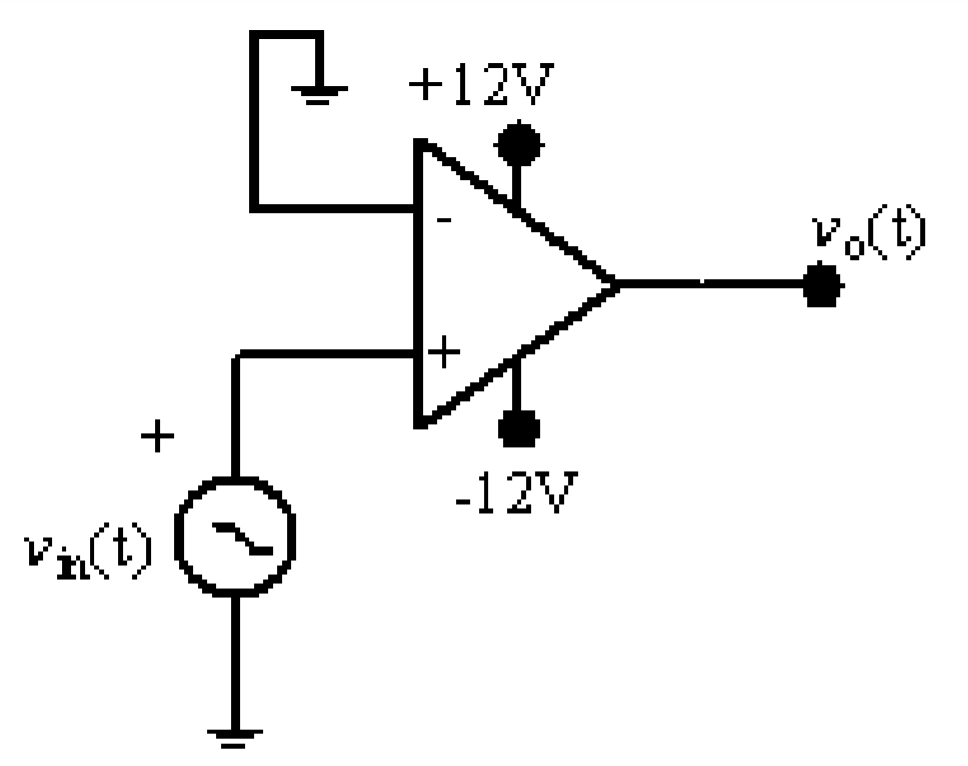
\includegraphics[width=0.4\textwidth]{circuit1.png}
   \caption{Circuit schematic for the Step 1 part a}
\end{figure} 
Then the \(V_{o} \) versus \( V_{in}\) graph ,given in Figure 2, plotted.
%Figure 2 basic comparator plot
\begin{figure}[H]
	\centering
   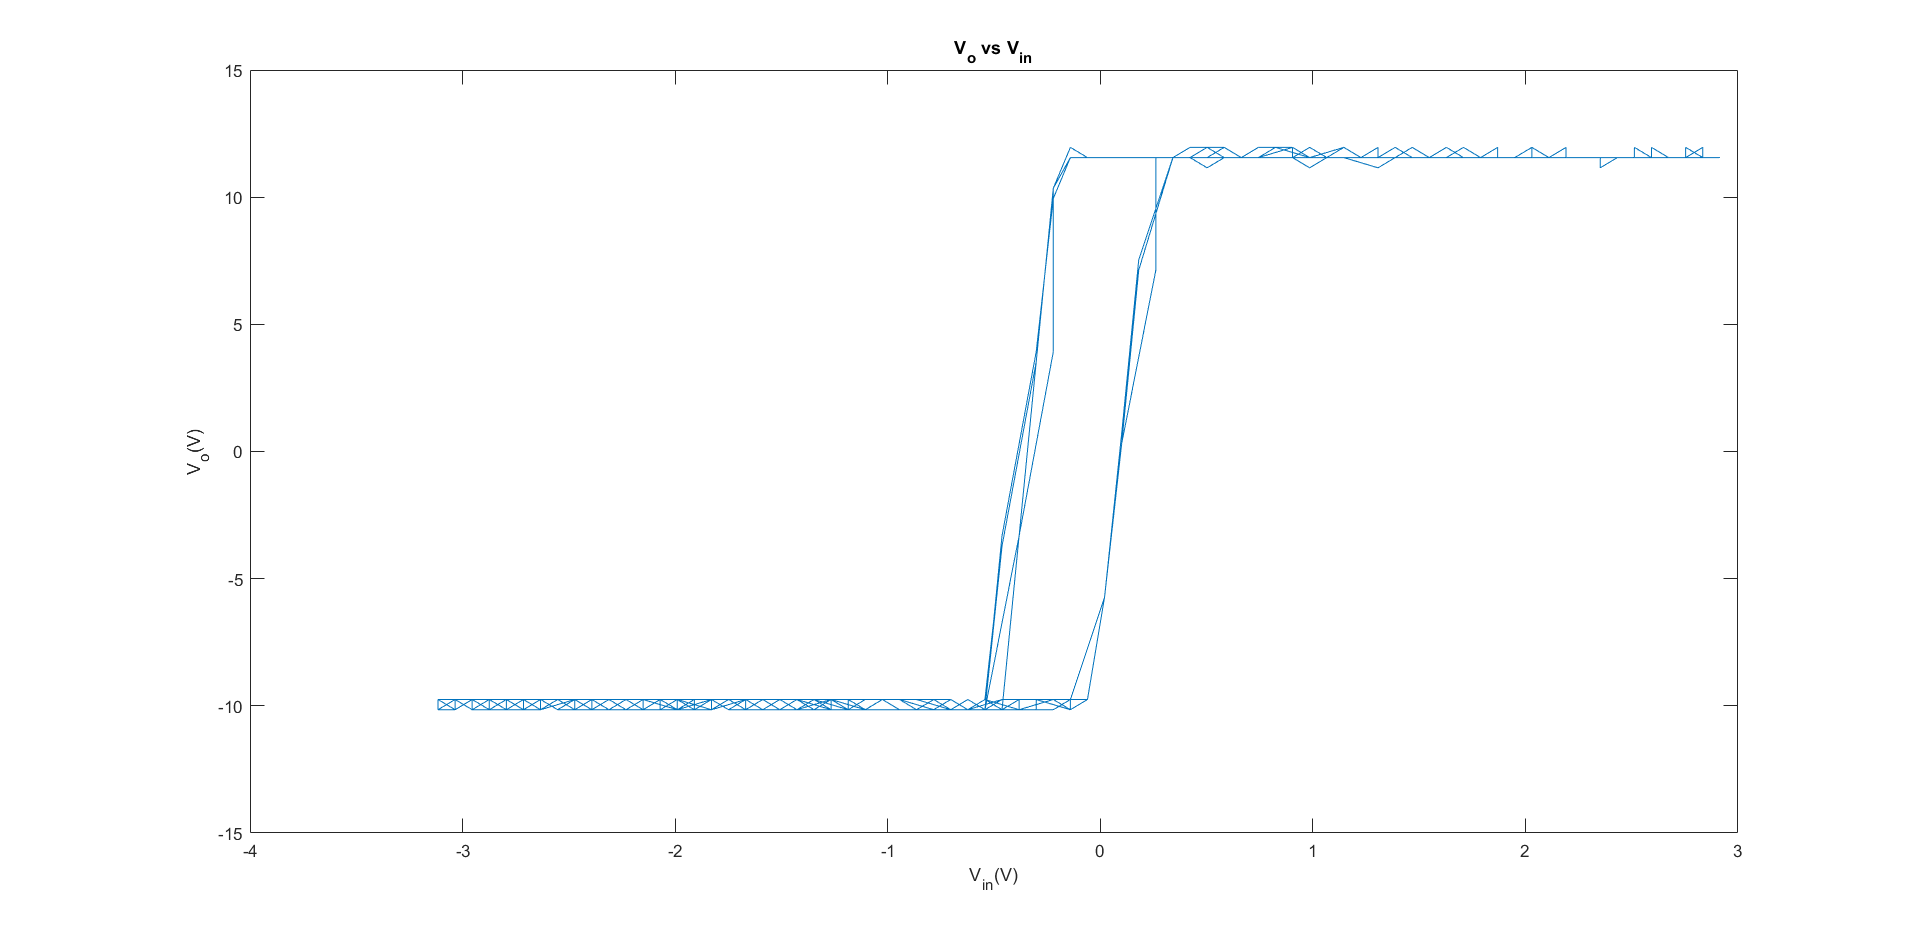
\includegraphics[width=1\textwidth]{e_1_a.png}
   \caption{\(V_{o} \) vs \( V_{in}\)}
\end{figure} 
It can be said that this Op-Amp configuration compares (with the ground) and amplifies the signal propagated to a non-inverting terminal. From the plot, there is an unexpected gap at the linear region, which is stemmed from the non-ideal behavior of the Op-Amp. 

%Figure 3 comparison simulation res
Basic comparator circuit is constructed in LTSpice environment as a part of preliminary work. The schematic is given in the Figure 3.
\begin{figure}[H]
	\centering
   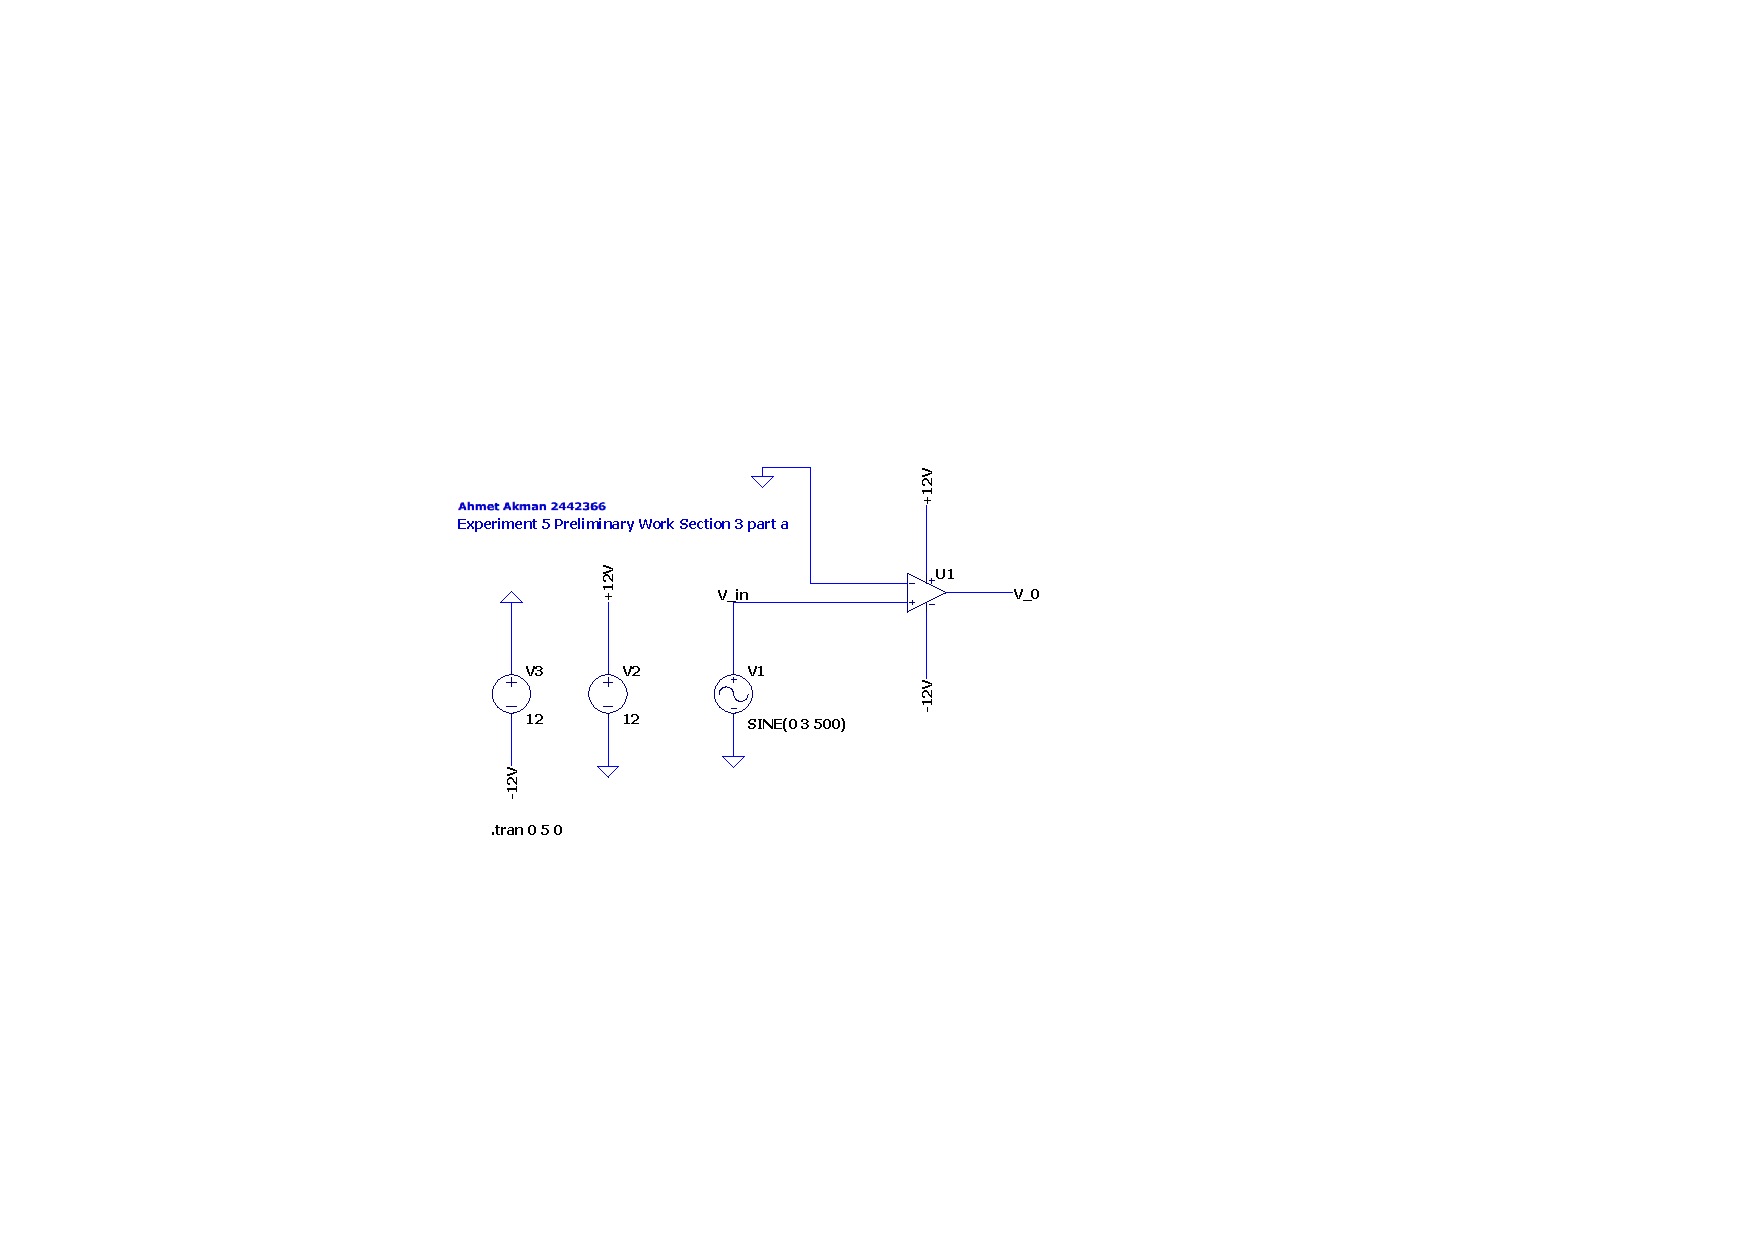
\includegraphics[width=0.8\textwidth]{BasicComparator_SCH.pdf}
   \caption{Circuit schematic for the basic comparator.}
\end{figure} 
Then plot given in Figure 4 is obtained.

\begin{figure}[H]
	\centering
   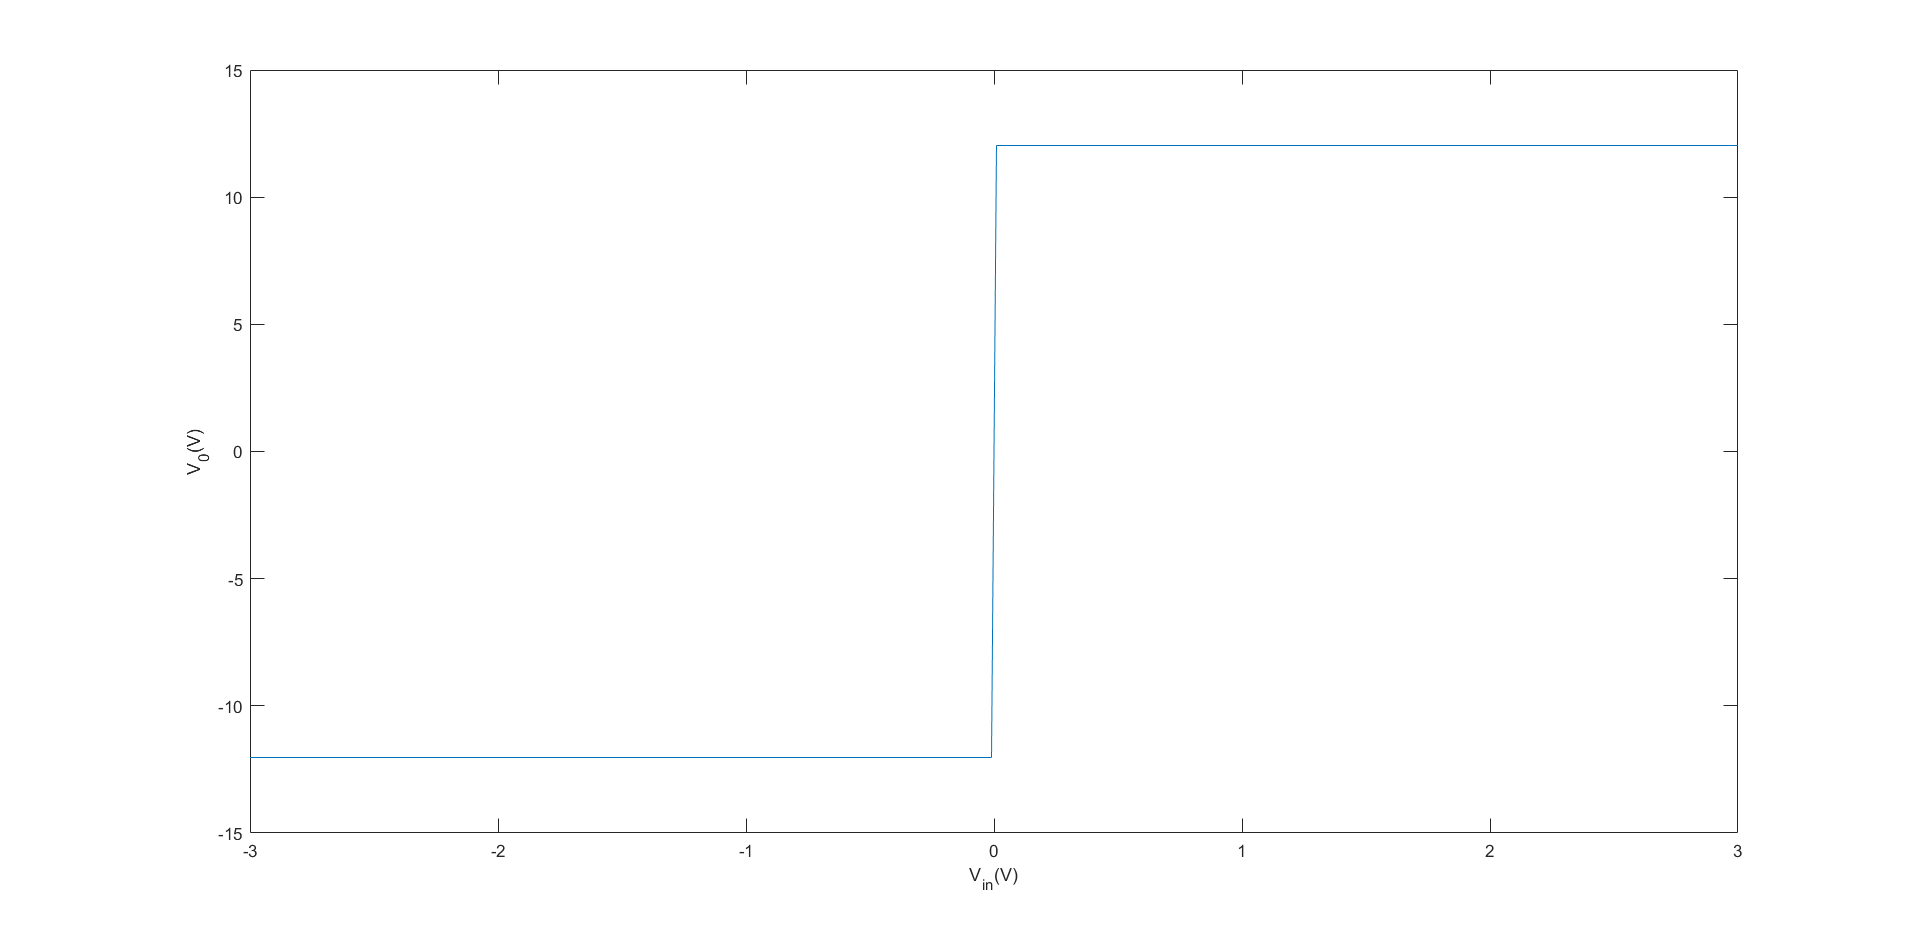
\includegraphics[width=1\textwidth]{3a_vs_vin.png}
   \caption{\(V_o\) vs \(V{in}\)}
\end{figure}
This result shows us the opamp model in the LTSpice simulation environment operates almost like an ideal Op-Amp. The difference between an ideal and a non-ideal Op-Amp can also be observed from Figures 2  and 4 so that the internal capacitance of the op-amp affects the linear region.

\subsubsection{b.}
%description script
The buffer circuit is set on a breadboard. The schematic given in Figure 5 is taken as the reference.
%Figure 5 buffer circuit
\begin{figure}[H]
	\centering
   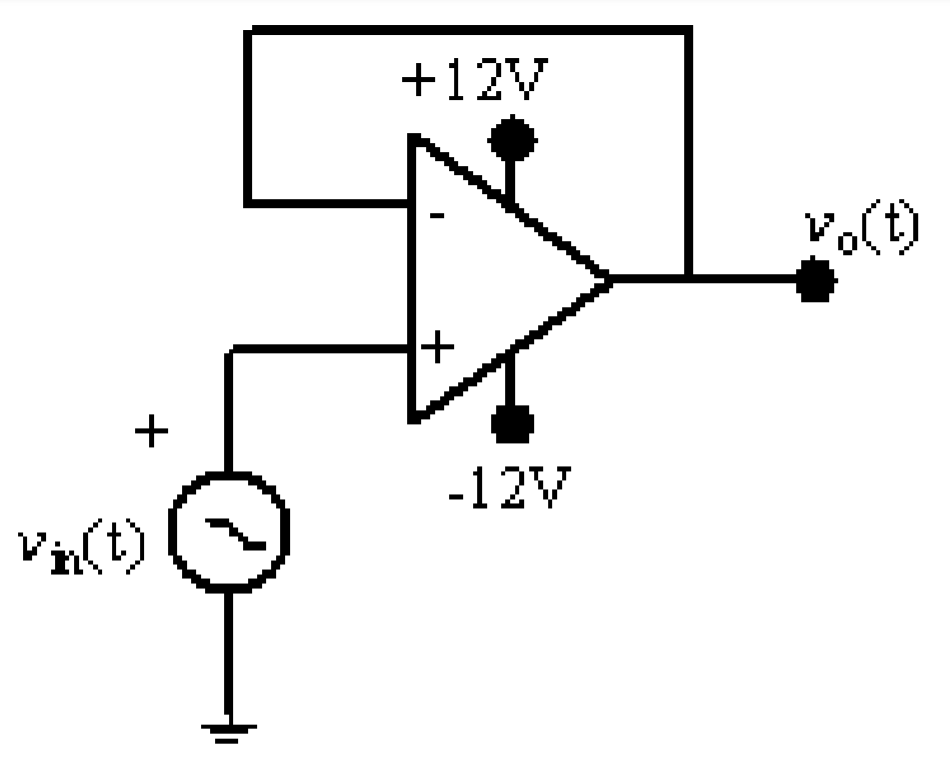
\includegraphics[width=0.4\textwidth]{circuit2.png}
   \caption{Circuit schematic for the Step 1 part b}
\end{figure} 
The \(V_{o} \) vs \( V_{in}\) plot is obtained. 
%Figure 5 buffer plot
\begin{figure}[H]
	\centering
   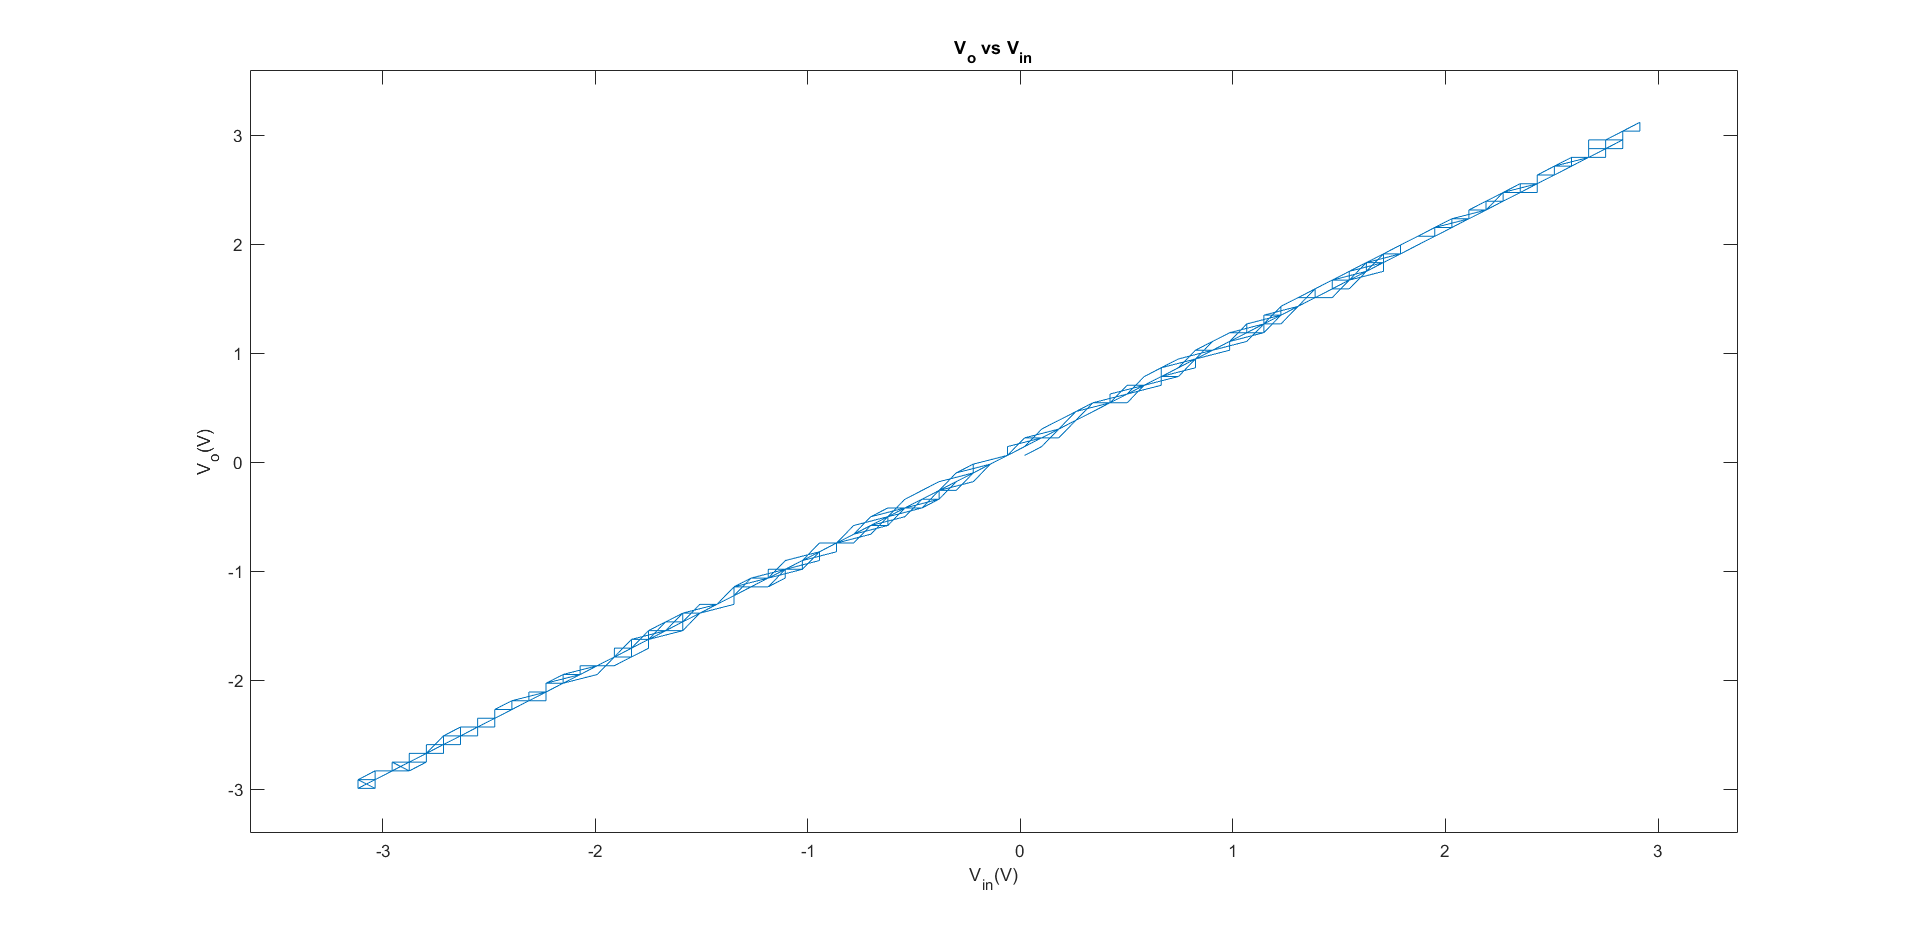
\includegraphics[width=1\textwidth]{e_1_b.png}
   \caption{\(V_{o} \) vs \( V_{in}\)}
\end{figure} 
As can be seen from the plot, the buffer circuit directly transfers the input voltage to its output terminal. This application can be used to isolate two circuits in order to prevent voltage drop at the source circuit since there is no flowing current. This is explained in Step 3 with an example. 

%Figure 7 comparison simulation res
Buffer circuit is constructed in LTSpice environment. The schematic is given in the Figure 7.
\begin{figure}[H]
	\centering
   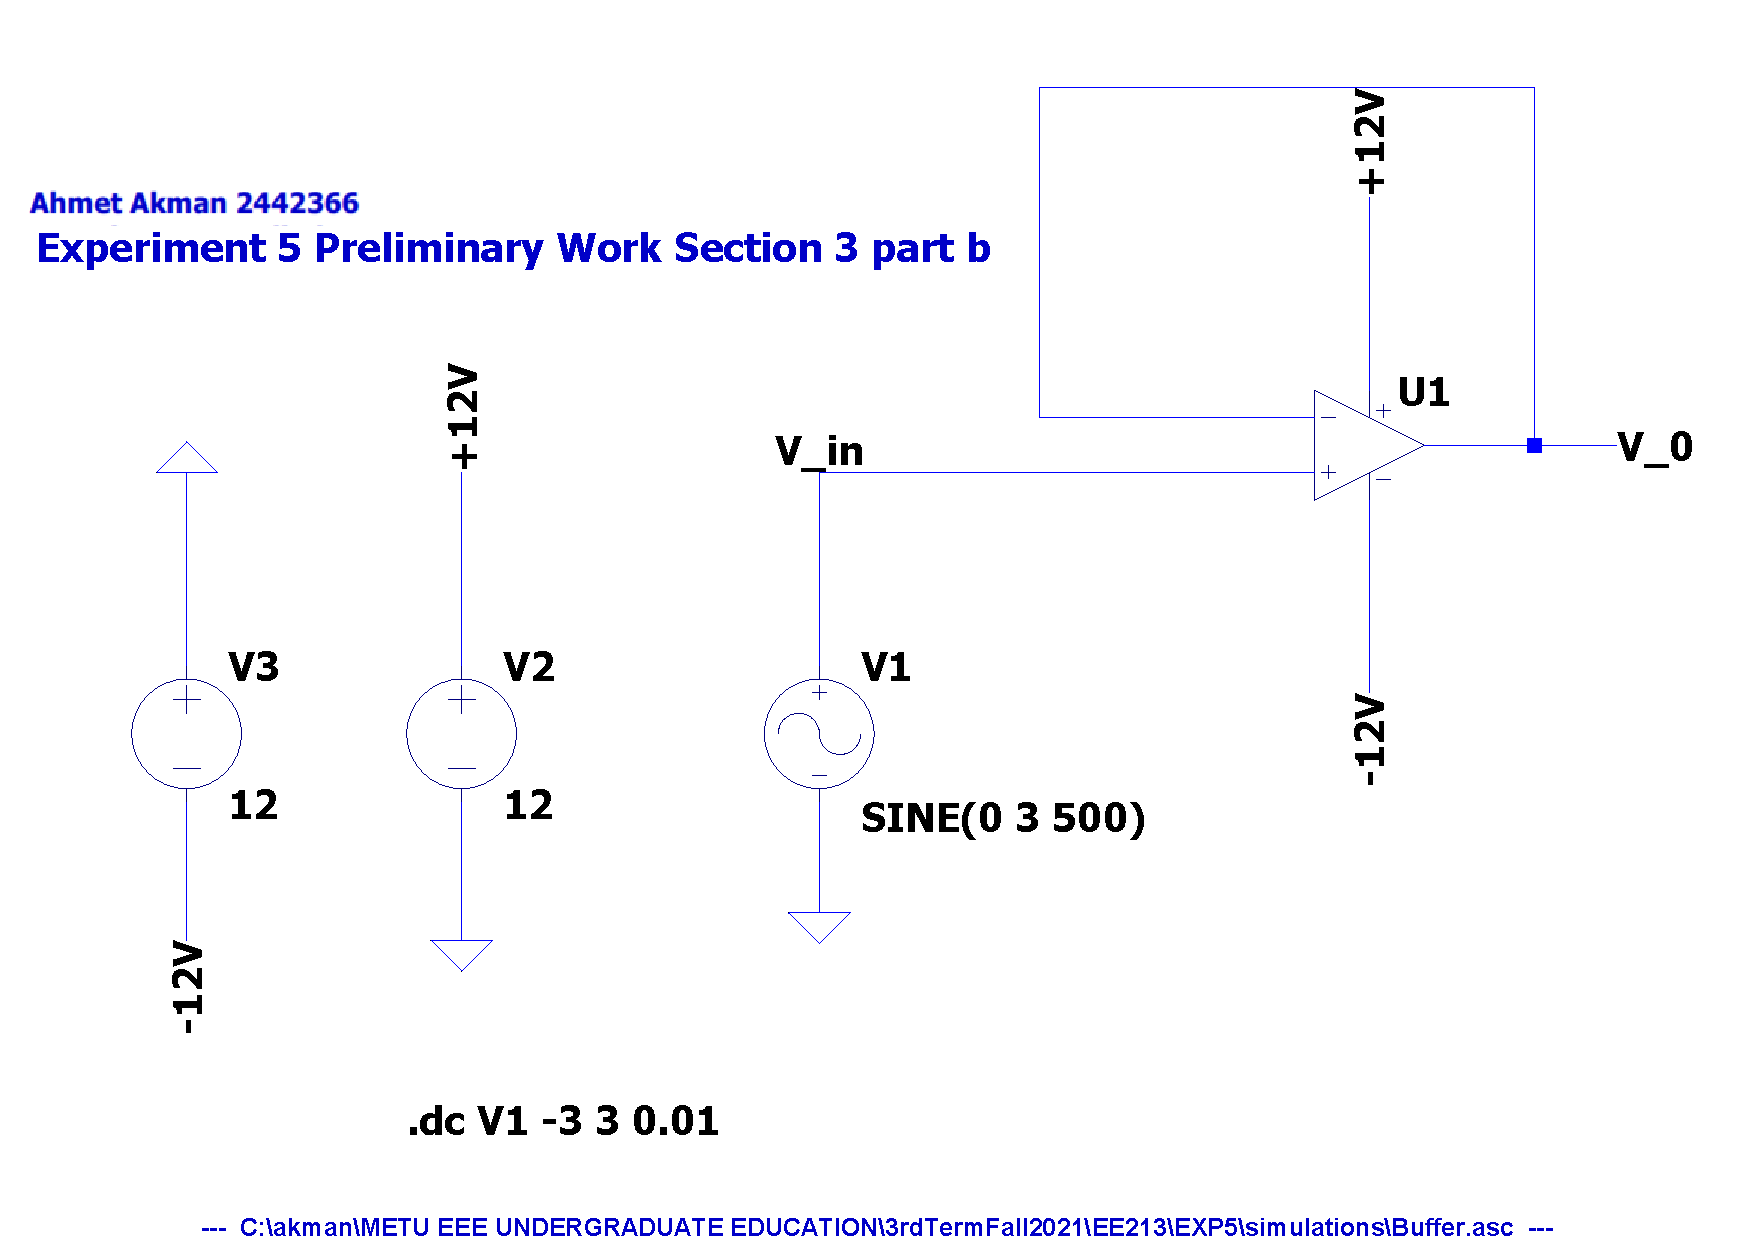
\includegraphics[width=0.8\textwidth]{Buffer_SCH.pdf}
   \caption{Circuit schematic for the buffer.}
\end{figure} 
Then plot given in Figure 8 is obtained.

\begin{figure}[H]
	\centering
   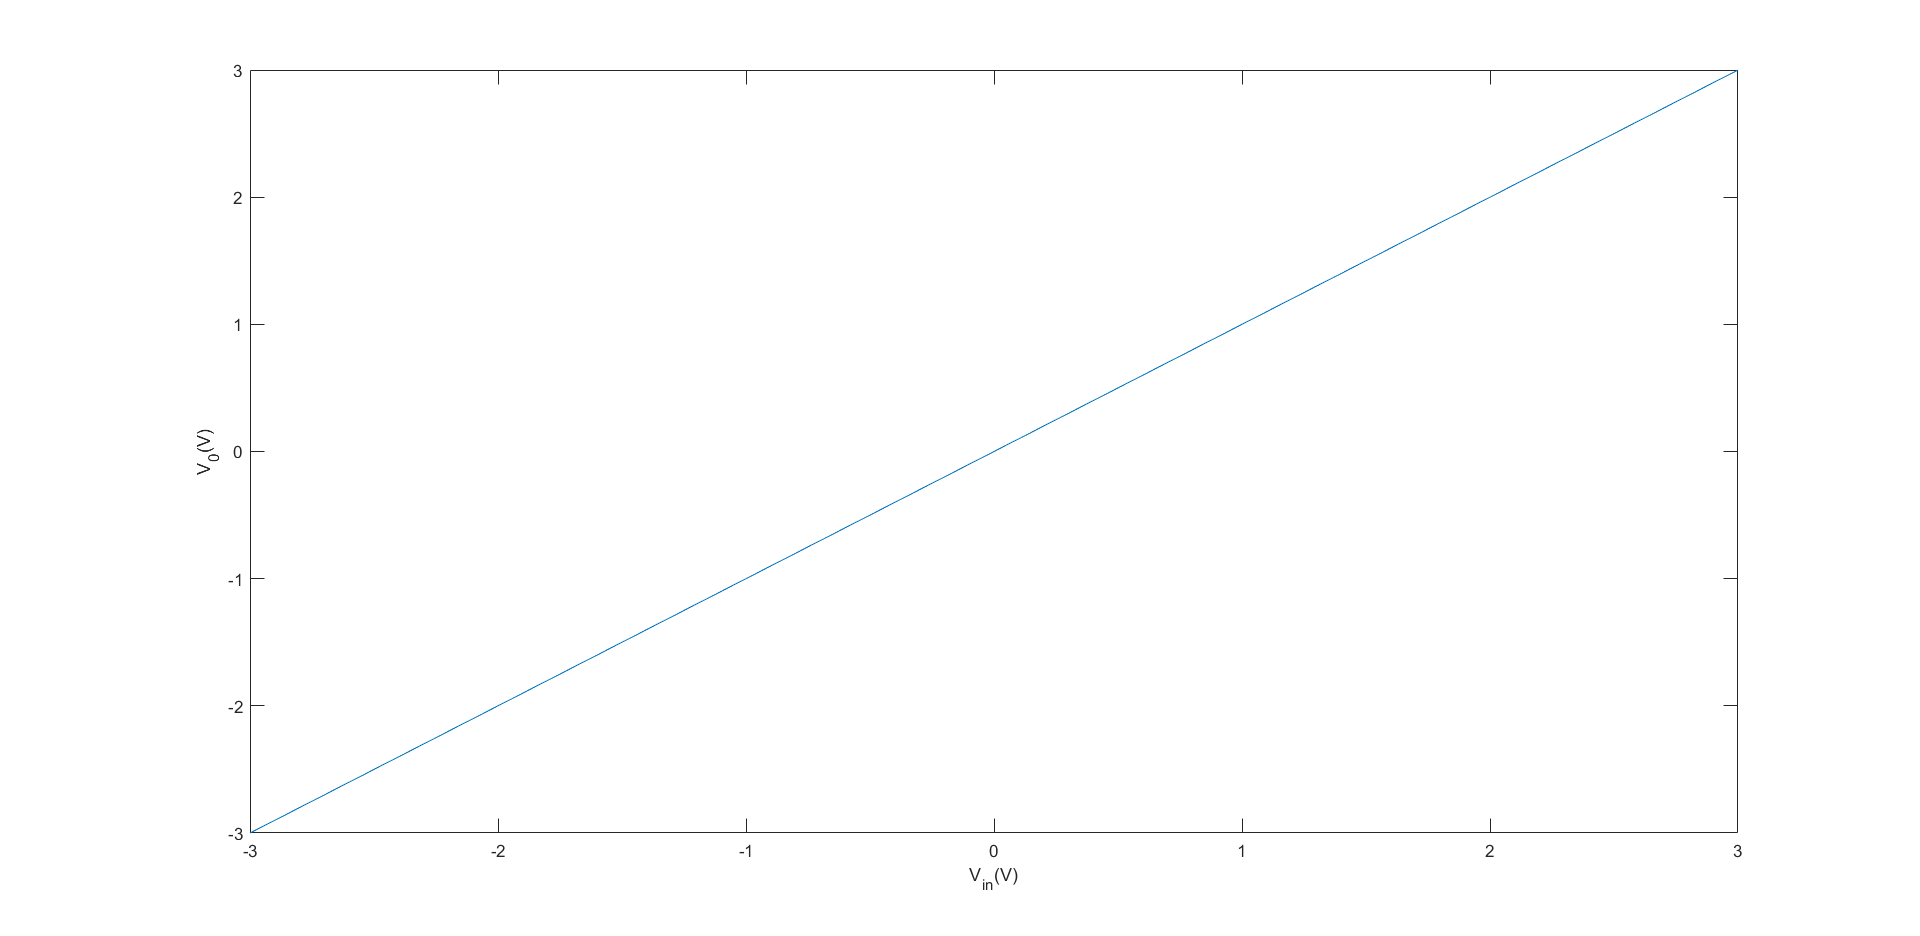
\includegraphics[width=1\textwidth]{3b_vs_vin.png}
   \caption{\(V_0\) vs \(V{in}\)}
\end{figure}
It can be said that the simulation plot is quite consistent with the real-world experiment plot for the buffer configuration.
\subsubsection{c.}
%description script
The non-inverting amplifier circuit is set on a breadboard at the laboratory. The schematic given in Figure 9 is taken as the reference.  


%Figure 9 non-inverting circuit
\begin{figure}[H]
	\centering
   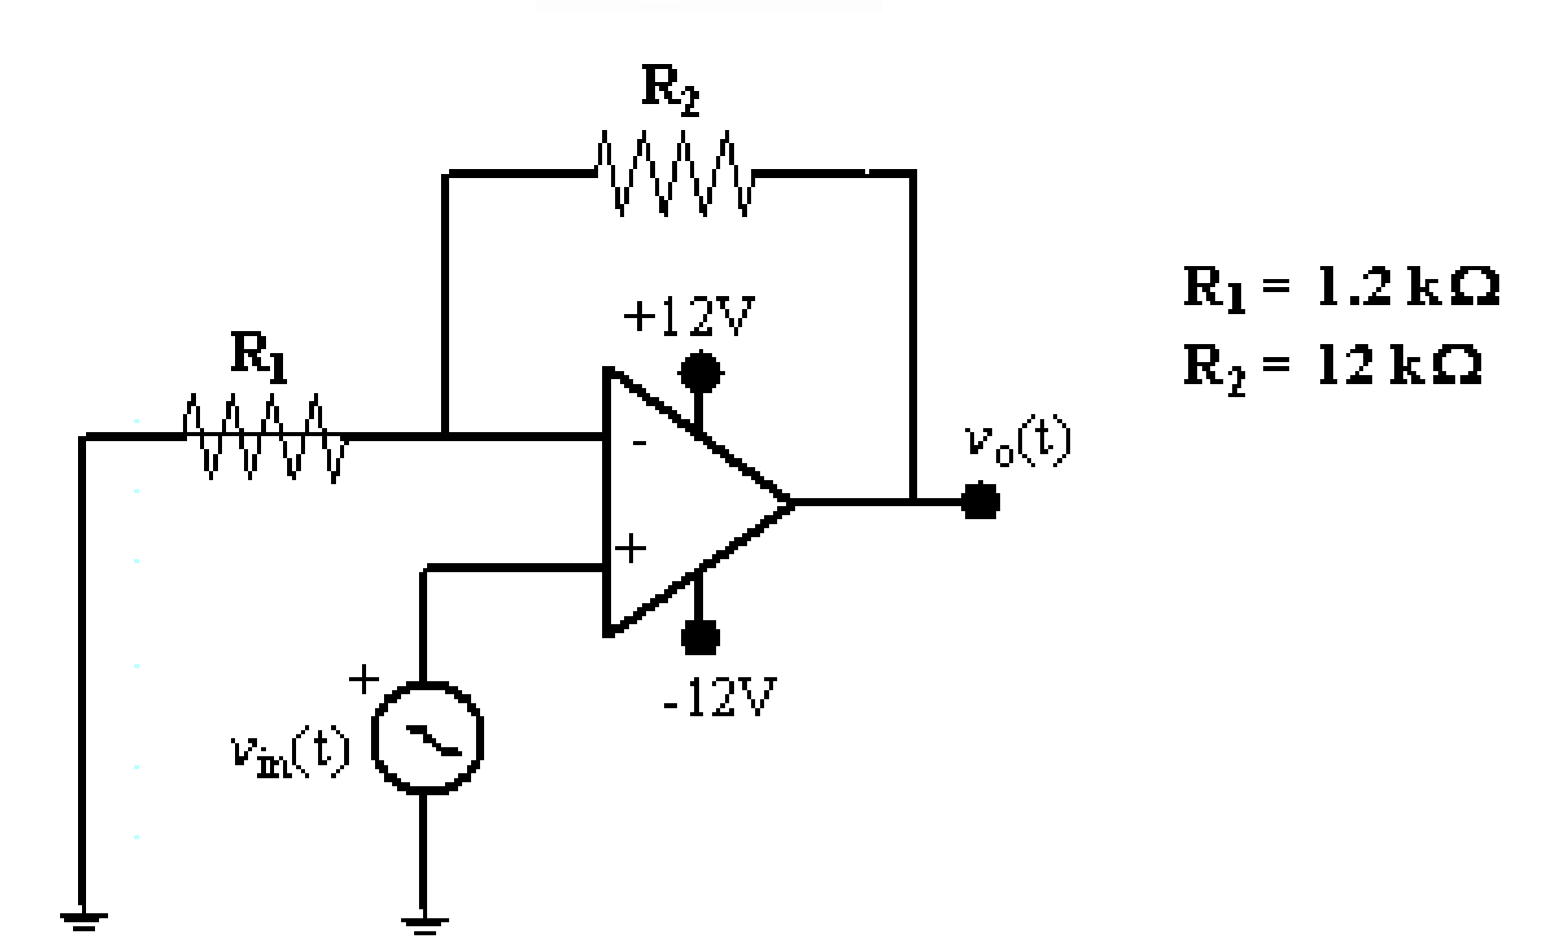
\includegraphics[width=0.6\textwidth]{circuit4.png}
   \caption{Circuit schematic for the Step 1 part c}
\end{figure} 
Then using both channel oscilloscope probes, measurements are made at the nodes \(V_{o} \) and \( V_{in}\). The plot is given in Figure 10.
%Figure 10 non-inverting plot 

\begin{figure}[H]
	\centering
   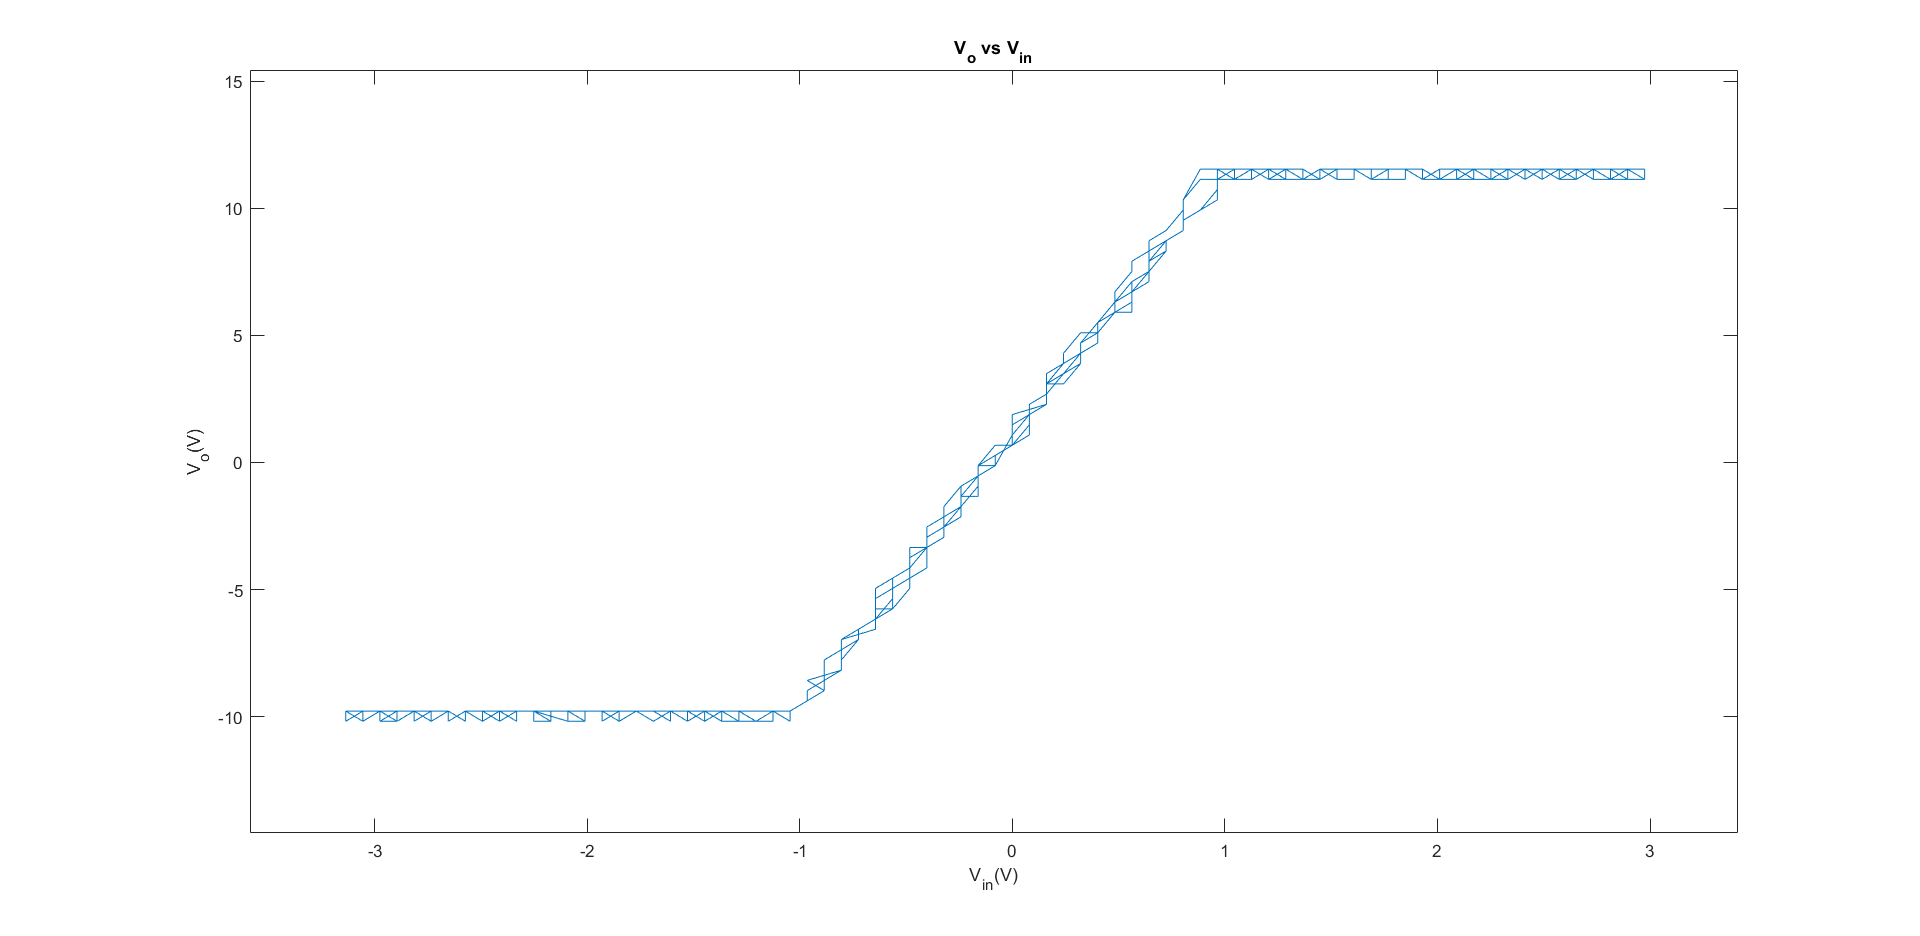
\includegraphics[width=1\textwidth]{e_1_c.png}
   \caption{\(V_{o} \) vs \( V_{in}\)}
\end{figure} 
The amplification rate can be measured by looking at the slope of the linear region. The slope is read as 11. It can be concluded that non-inverting configuration directly amplifies the signal at the non-inverting terminal according to the relation \[\frac{V{out}}{V{in}} =1+ \frac{R_2}{R_1}\] in linear region as expected.
%Figure 11 comparison simulation res
Non-inverting amplifier circuit is constructed in LTSpice environment. The schematic is given in the Figure 11.
\begin{figure}[H]
	\centering
   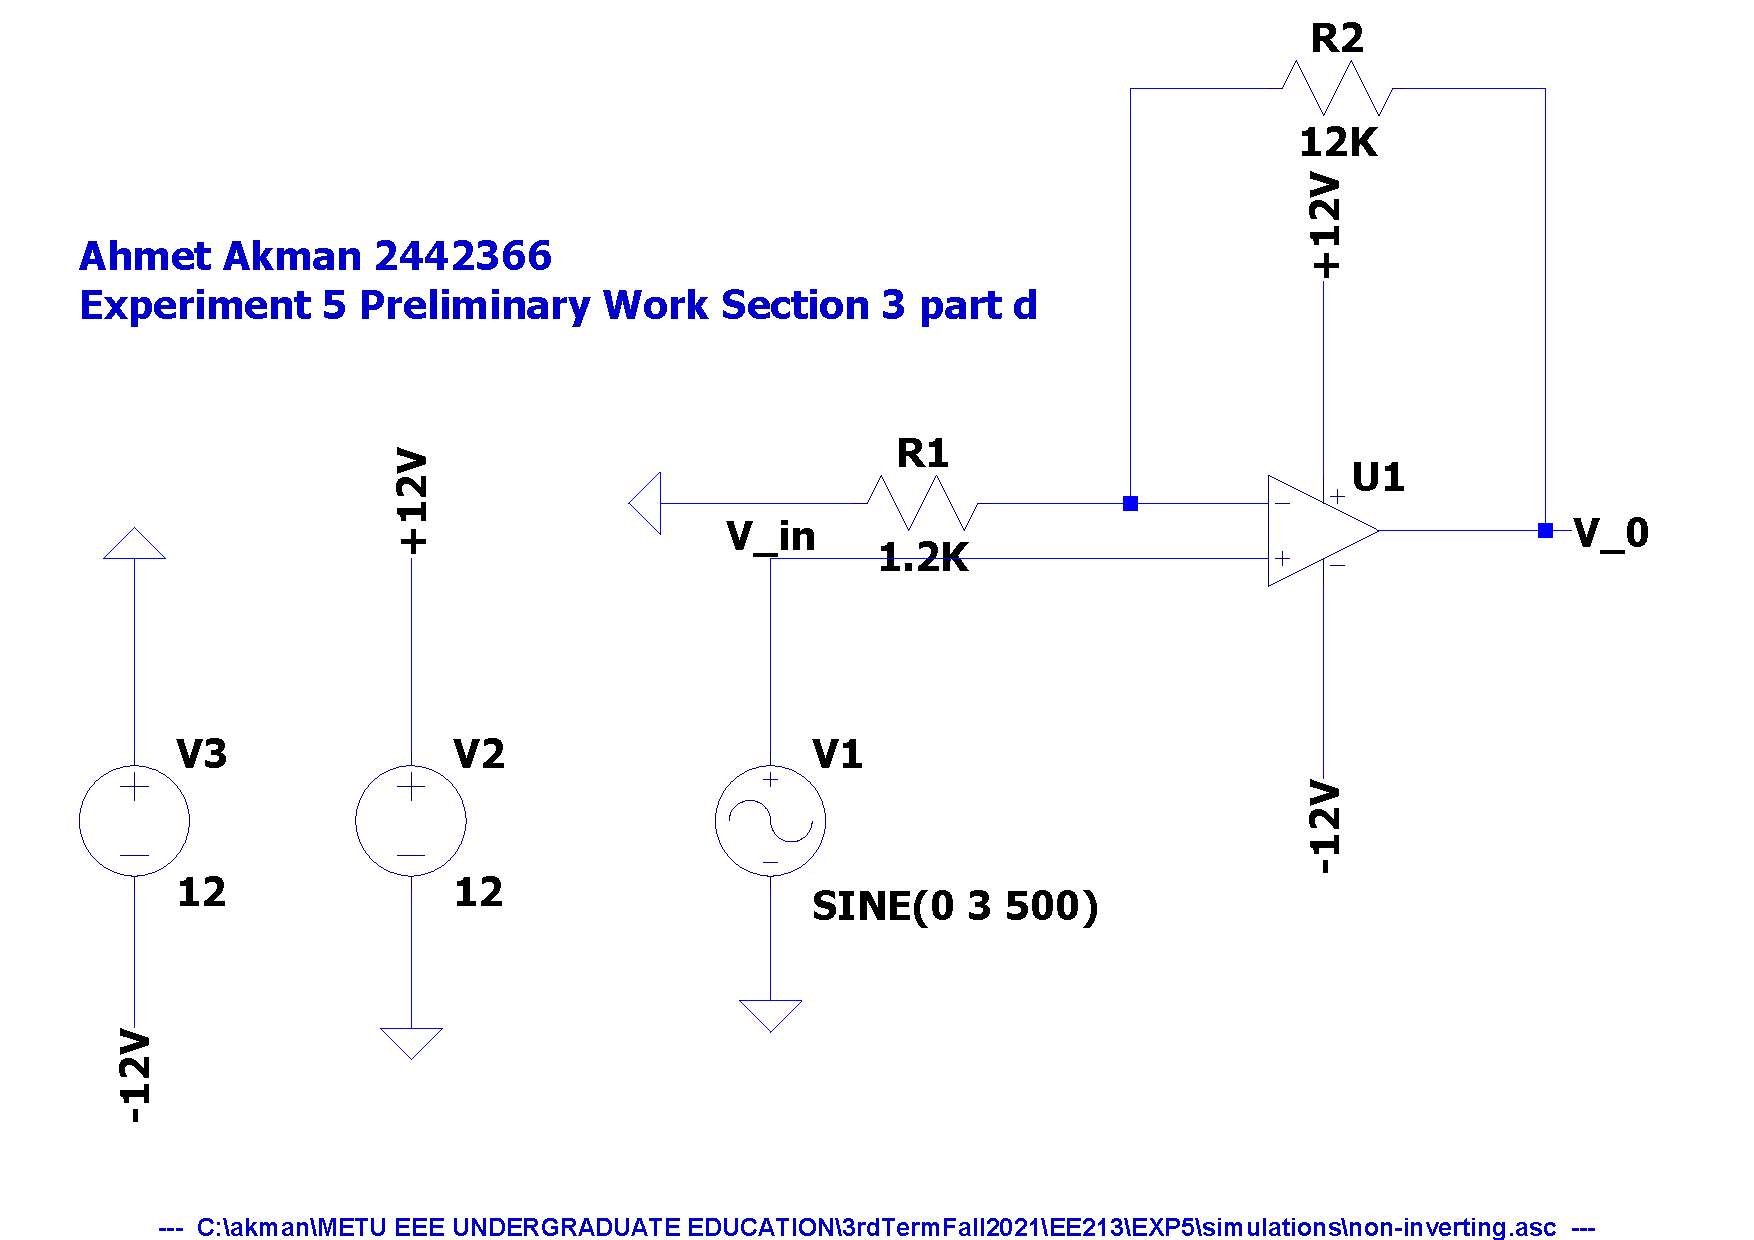
\includegraphics[width=0.8\textwidth]{non-inverting_SCH.pdf}
   \caption{Circuit schematic for the non-inverting amplifier.}
\end{figure} 

Then plot given in Figures 12 is obtained from simulation environment.

\begin{figure}[H]
	\centering
   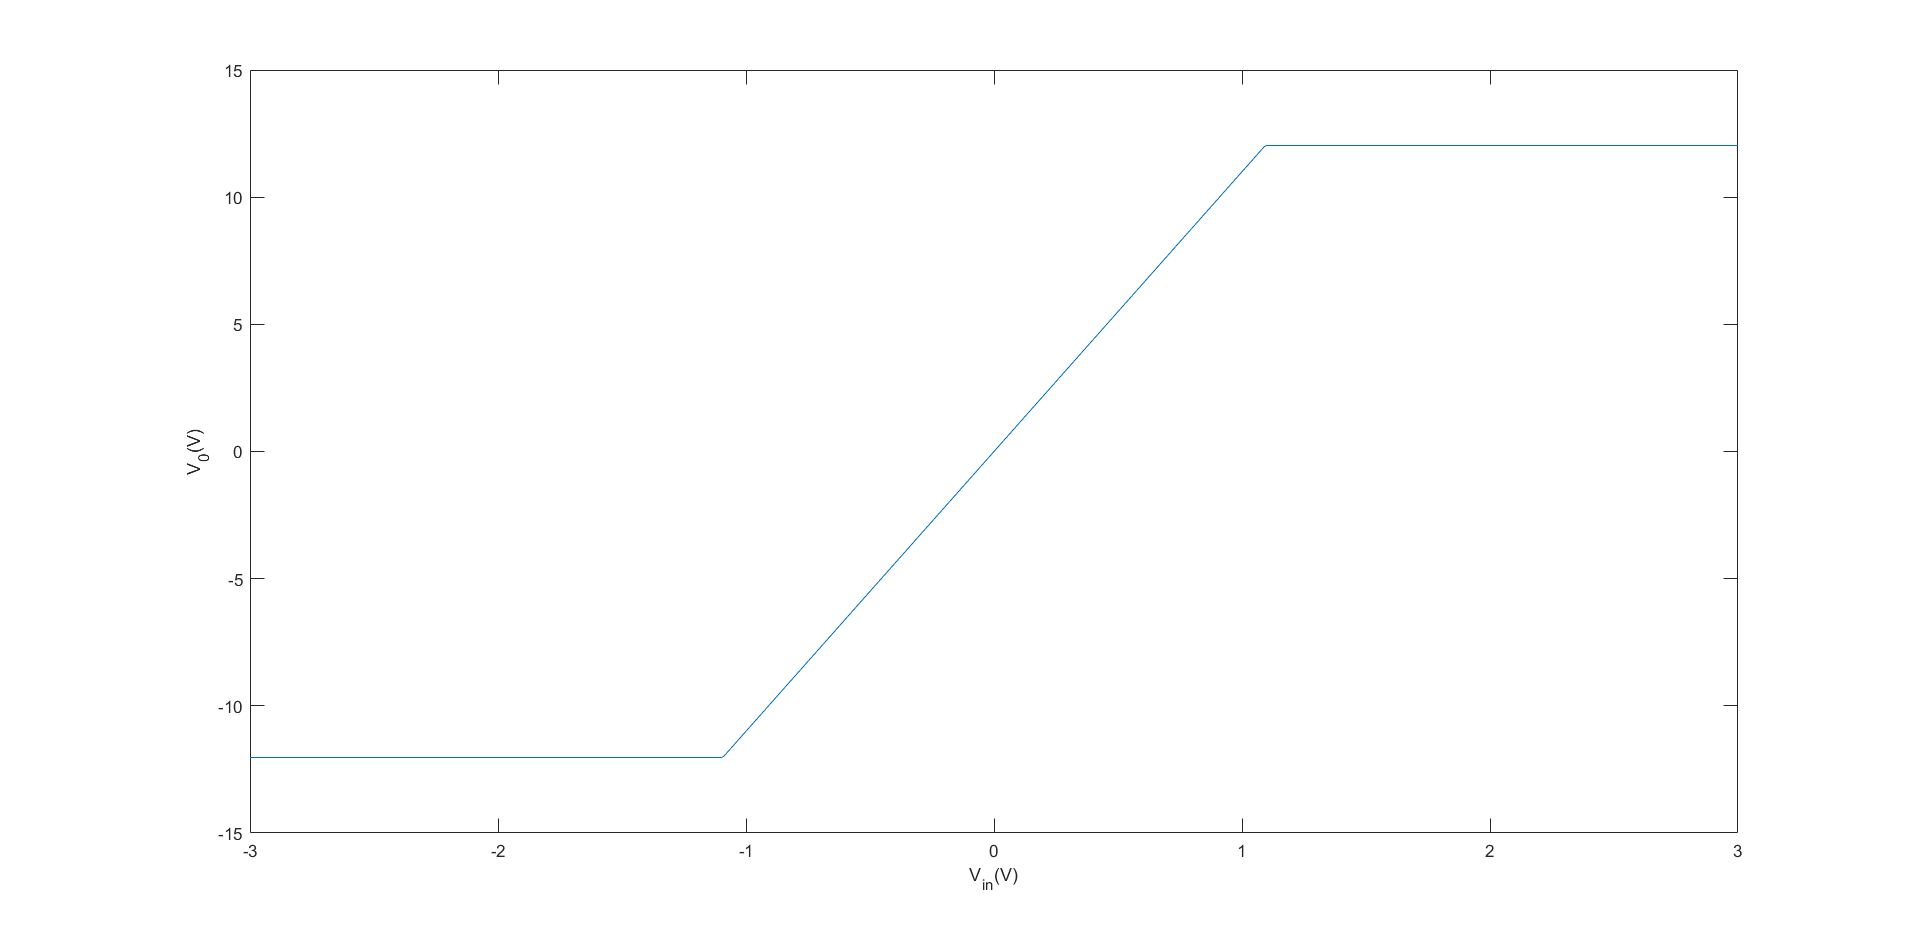
\includegraphics[width=1\textwidth]{3d_vs_vin.png}
   \caption{\(V_0\) vs \(V{in}\)}
\end{figure}
By looking at the shape of Figure 10 and Figure 11, it can be said that the behavior is consistent. But, the negative saturation region of the real circuit is slightly greater. This is predicted to be stemmed from the non-ideality of either the LM741 component or the negative power line of the power supply.
\subsection{Step 2}
%description script
The inverting amplifier circuit is constructed at the laboratory according to the schematic given in Figure 13.  

%Figure 10 inverting circuit
\begin{figure}[H]
	\centering
   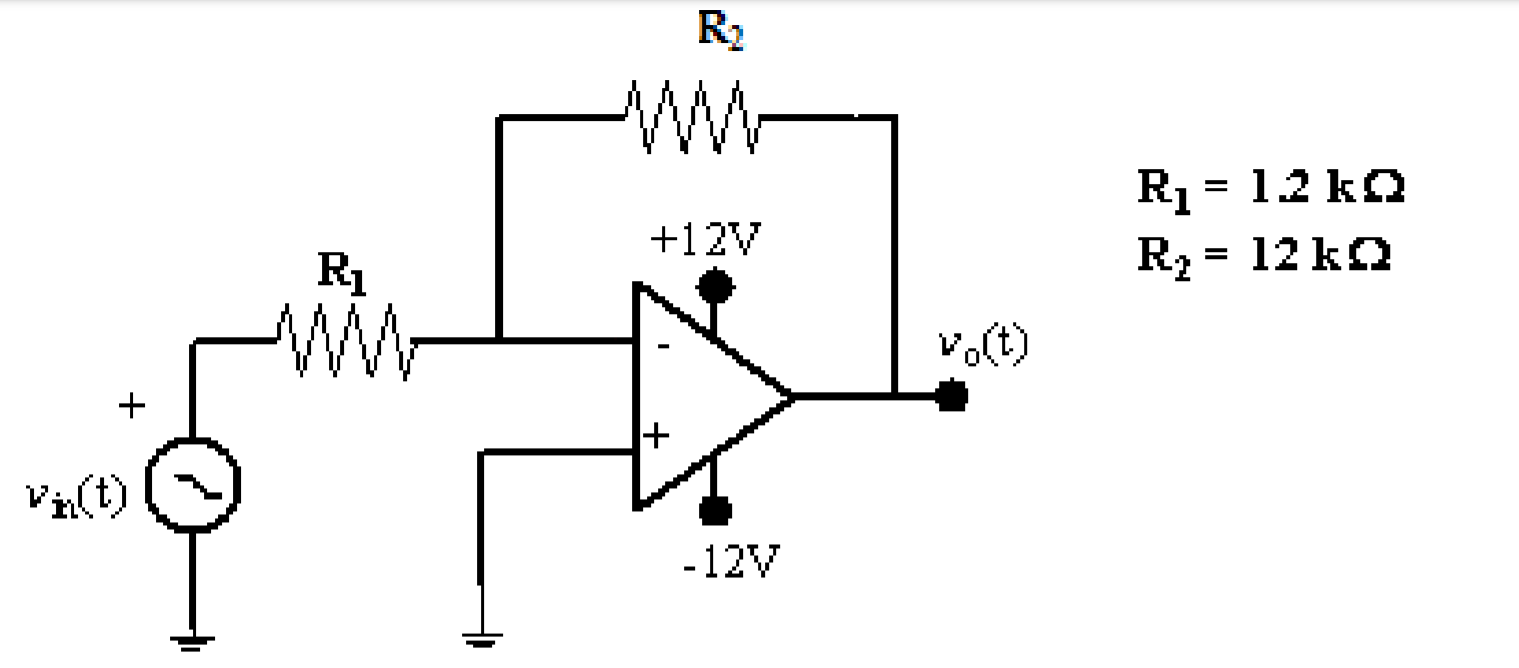
\includegraphics[width=0.6\textwidth]{circuit3.png}
   \caption{Circuit schematic for the Step 2}
\end{figure} 
The measurement are made using first and second channels of oscilloscope instrument. Therefore, the plot in Figure 14 describes \(V_{o} \) vs \( V_{in}\) relation is obtained.
%Figure 14 inverting plot
\begin{figure}[H]
	\centering
   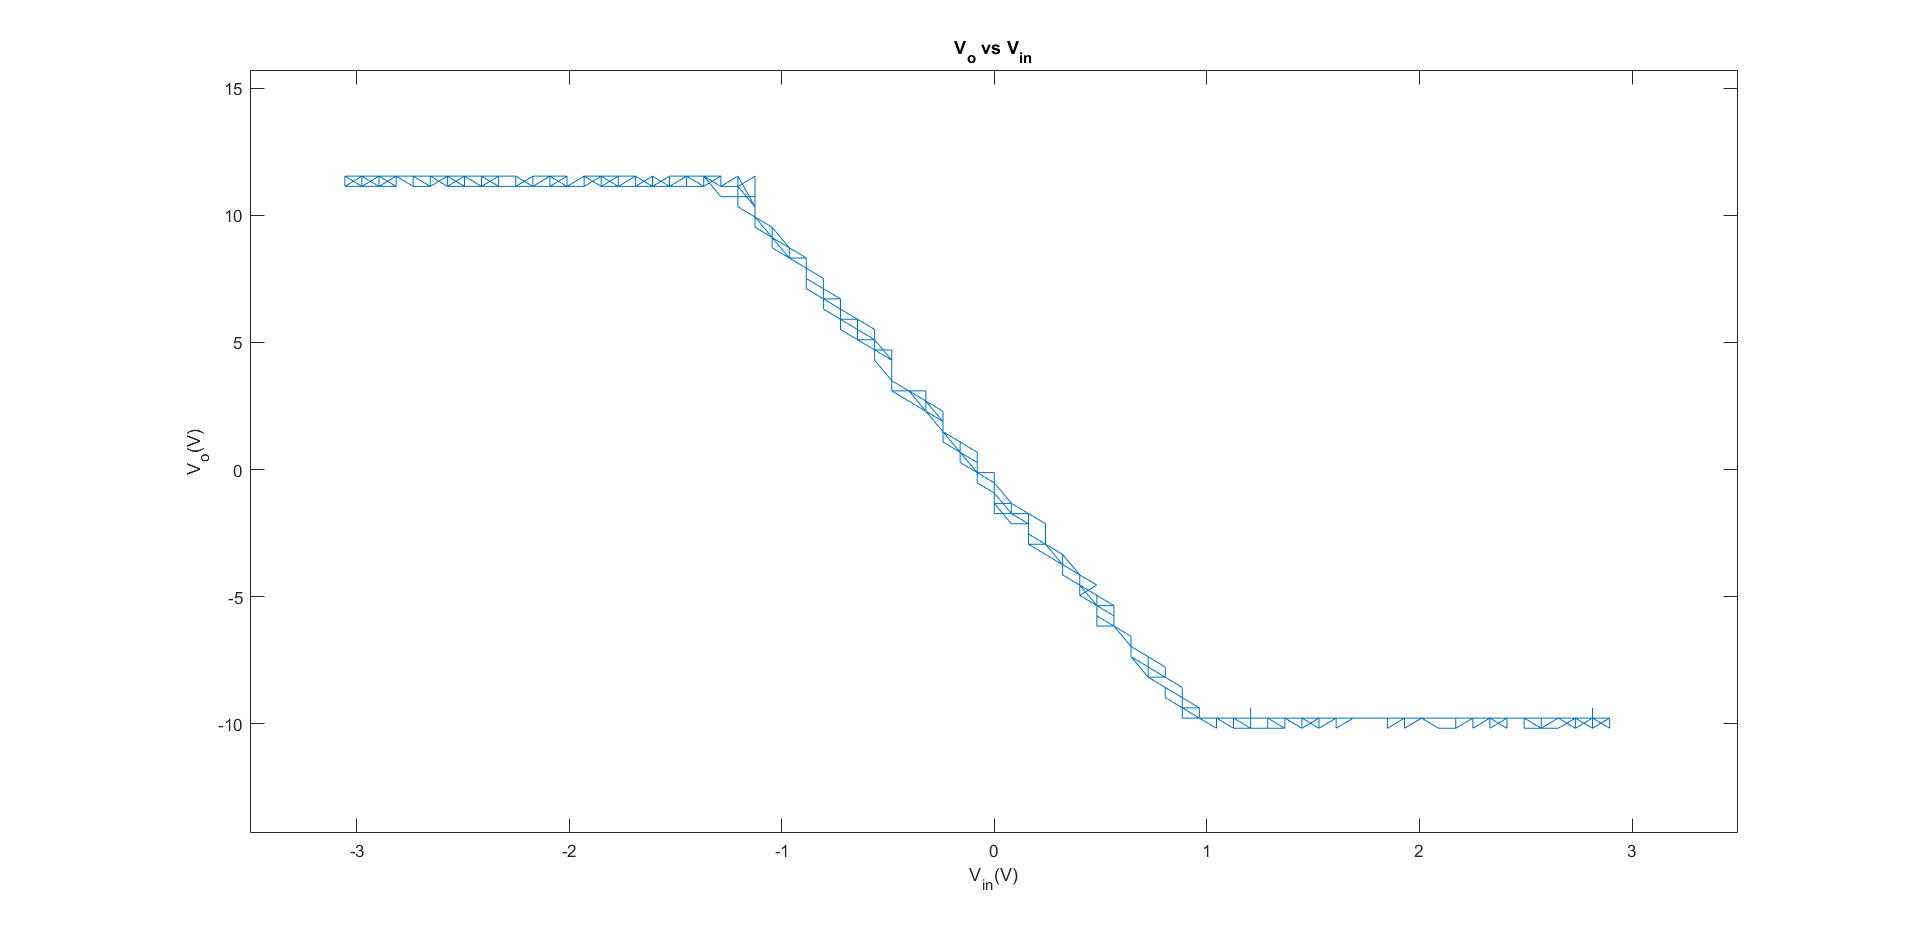
\includegraphics[width=1\textwidth]{e_2.png}
   \caption{\(V_{o} \) vs \( V_{in}\)}
\end{figure} 
It can be inferred that the operational amplifier amplifies the signal at the inverting channel by inverting. To obtain the expression relating the output voltage \(V_0 (t)\) to the input voltage \(V_{in} (t)\) of an inverting amplifier setup, the circuit in Figure 13 is taken as the reference. Then current through input terminals and the voltage of those terminals are taken as 0 since it is an ideal amplifier. So the circuit simplifies into two terminals and two resistors. Then the following simplifications are followed.
\[\frac{V{in} - 0 }{R_1} = i\]
\[\frac{0 - V{o} }{R_2} = i\]
So, the relation becomes as,
\[\frac{V{out}}{V{in}} = -\frac{R_2}{R_1}\]
Therefore it seems linear region of the plot given in Figure 14 approximately corresponds measurements. Which the signal is amplified by multiplying -11.
%Figure 12 comparison simulation res
Inverting amplifier circuit is constructed in LTSpice environment. The schematic is given in the Figure 15.
\begin{figure}[H]
	\centering
   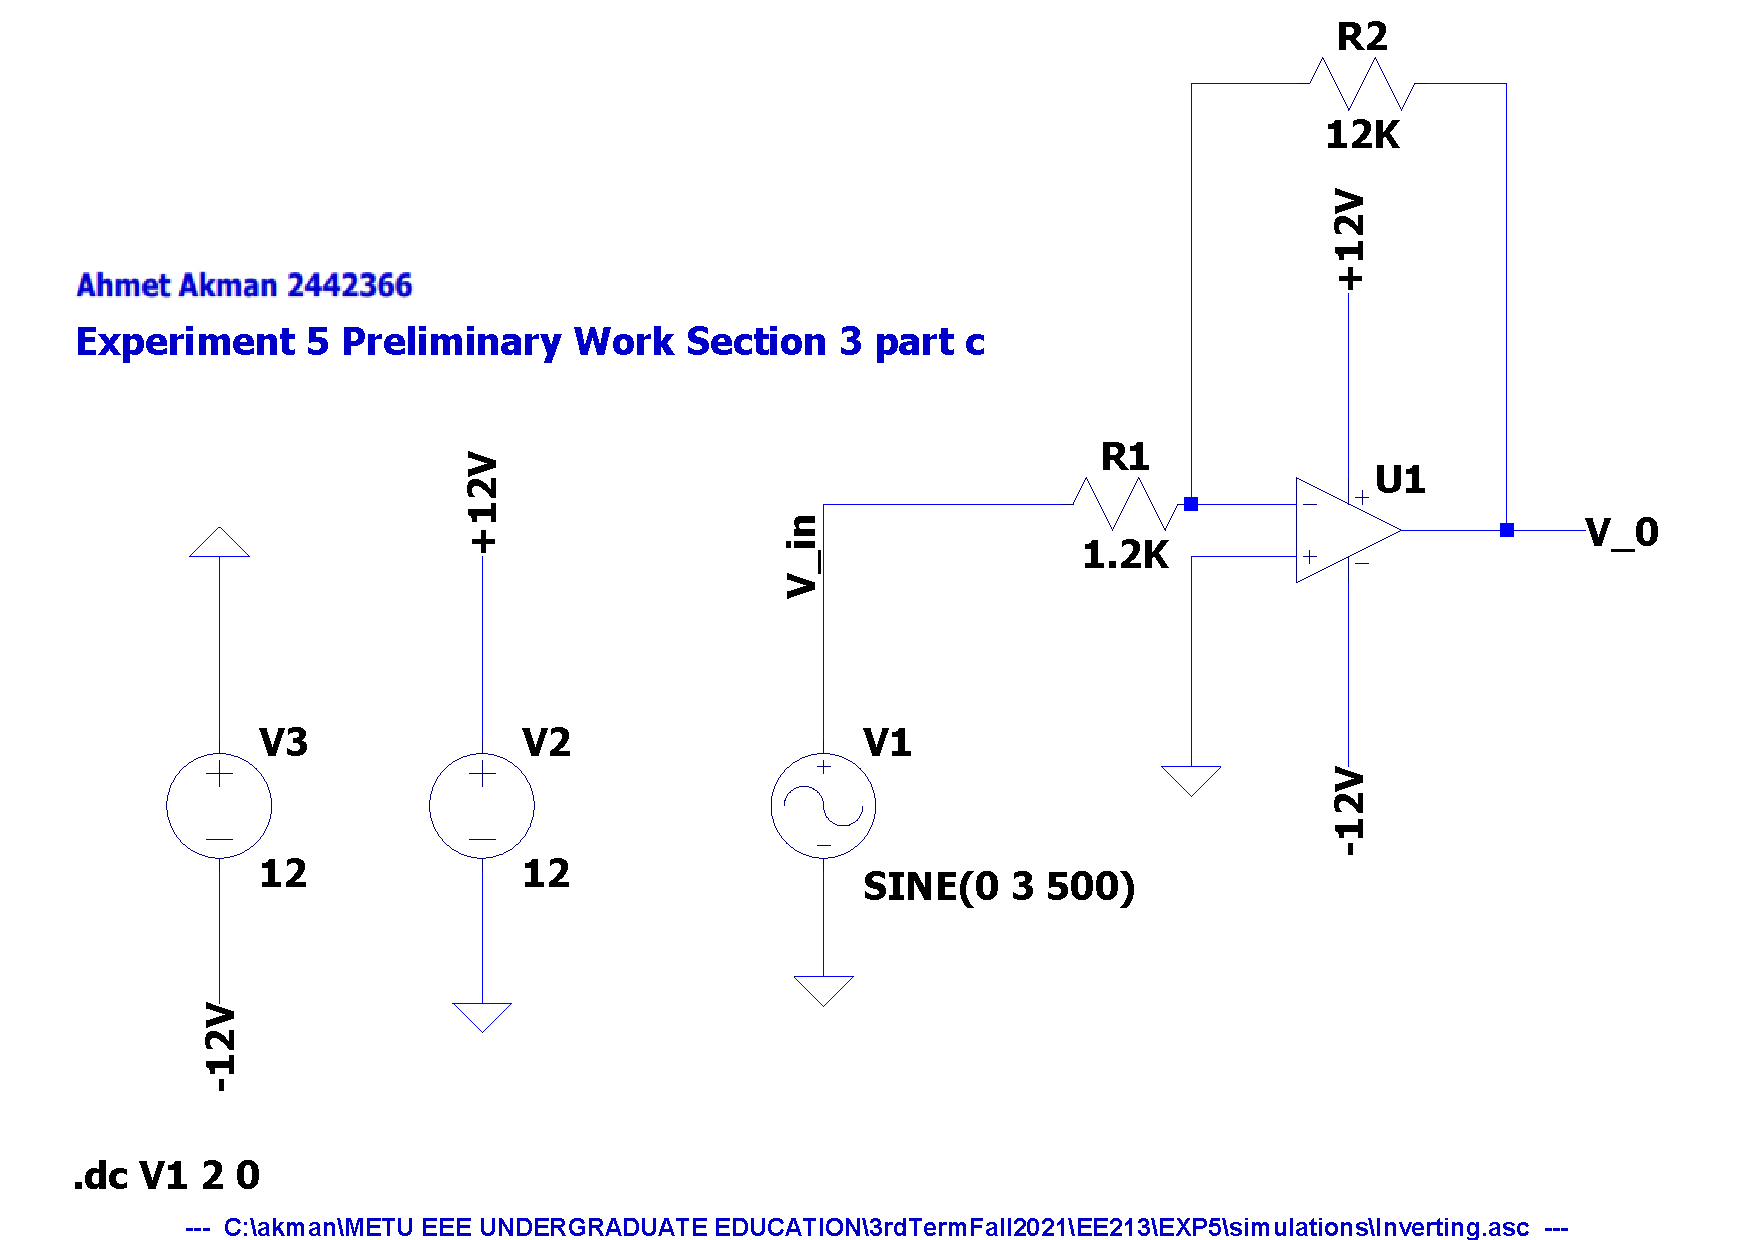
\includegraphics[width=1\textwidth]{Inverting_SCH.pdf}
   \caption{Circuit schematic for the inverting amplifier.}
\end{figure} 
Then plot given in Figure  16 is obtained.

\begin{figure}[H]
	\centering
   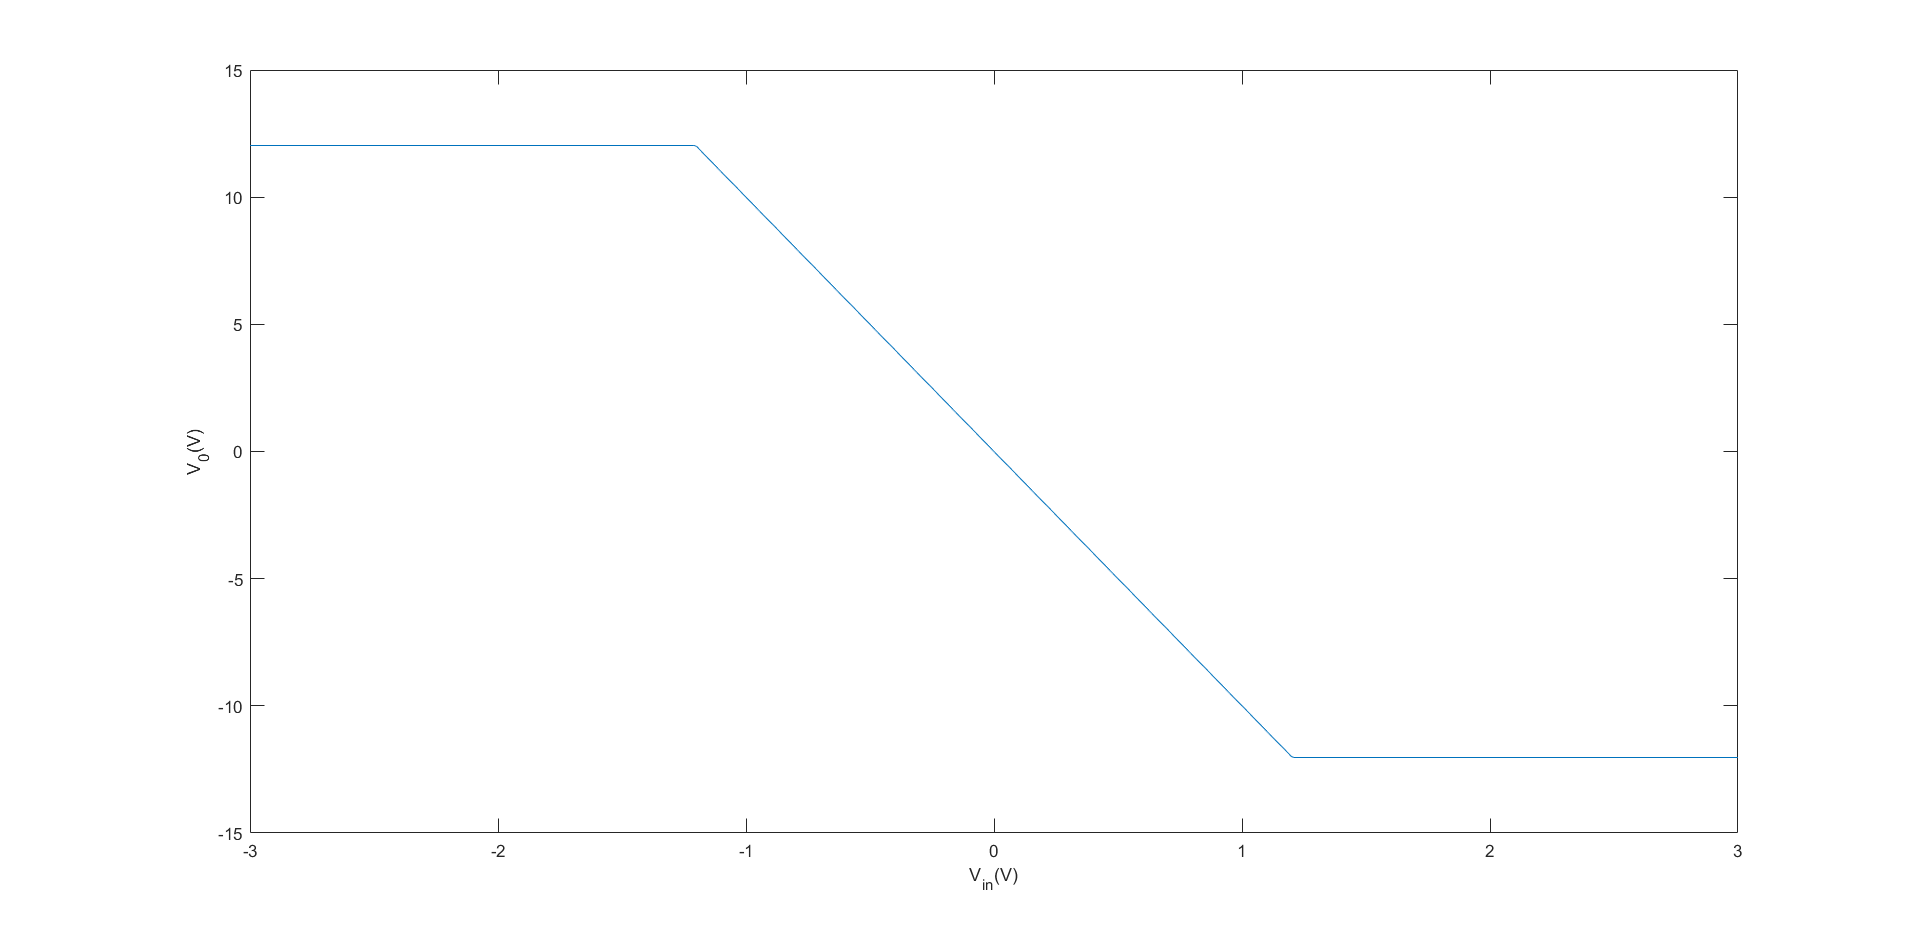
\includegraphics[width=1\textwidth]{3c_vs_vin.png}
   \caption{\(V_0\) vs \(V{in}\)}
\end{figure}
By evaluating the results of Figure 10 and Figure 11, it can be said that the behavior is consistent.
\subsection{Step 3}
%description script
In step 3, the circuit given in Figure 17 is constructed. But since there was only one signal generator, two signals with different amplitudes needed to be obtained using circuitry.
%Figure 17 summing+buffer circuit
\begin{figure}[H]
	\centering
   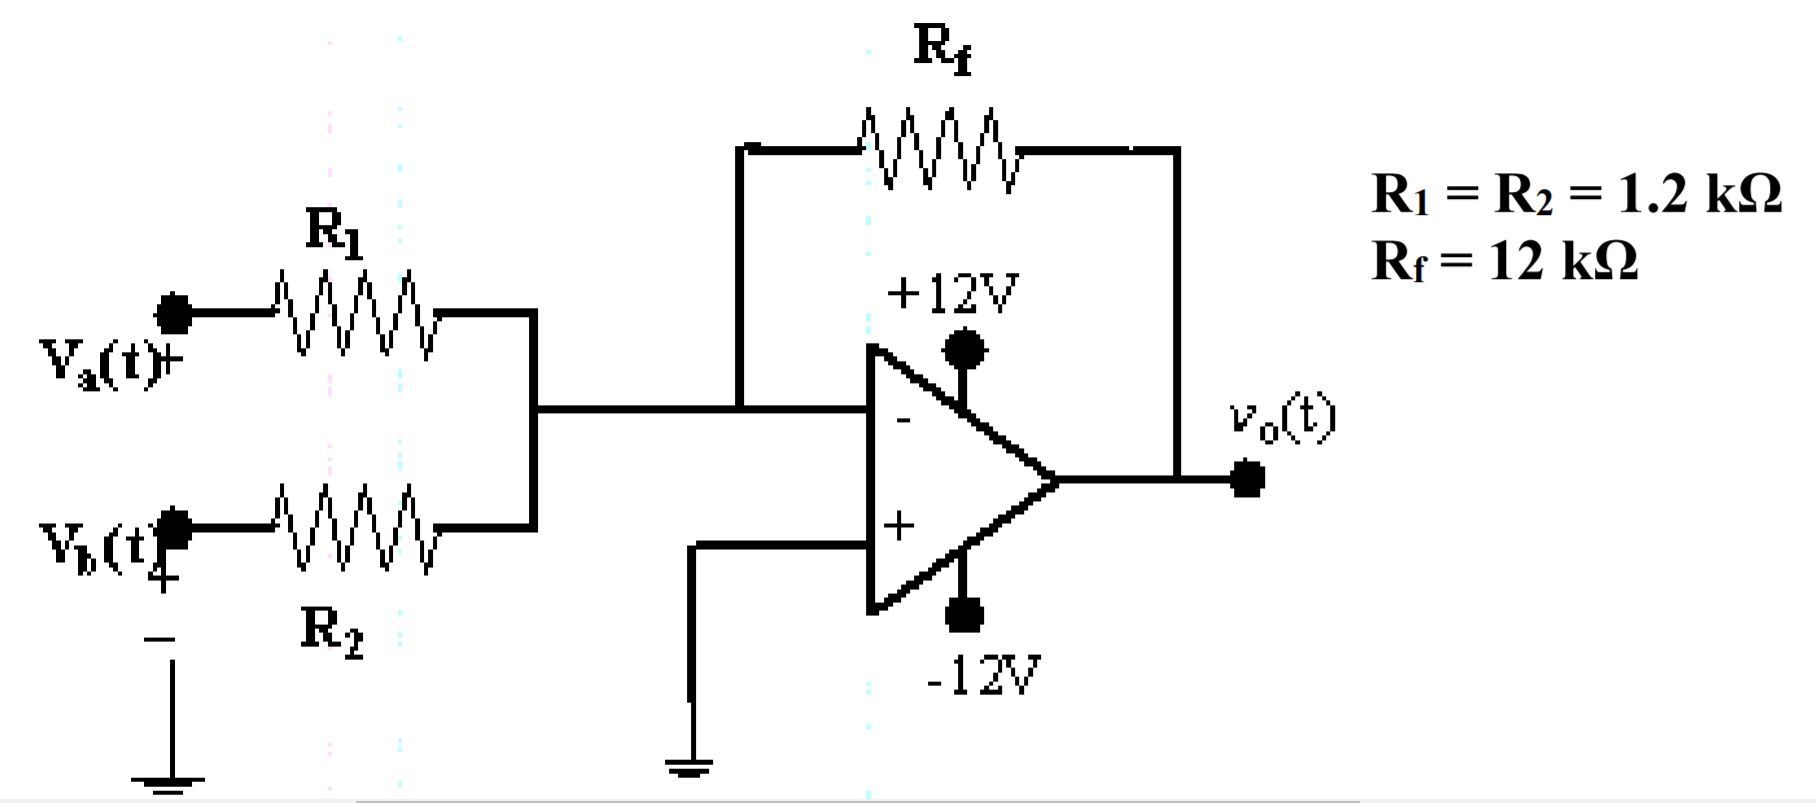
\includegraphics[width=0.6\textwidth]{circuit5.png}
   \caption{Circuit schematic for the Step 3}
\end{figure} 
\subsubsection{Voltage Divider and Buffer Circuit}
Since there is a need to get half of the signal voltage divider circuit is set. The general illustration of a voltage divider is given in Figure 18.
\begin{figure}[H]
	\centering
   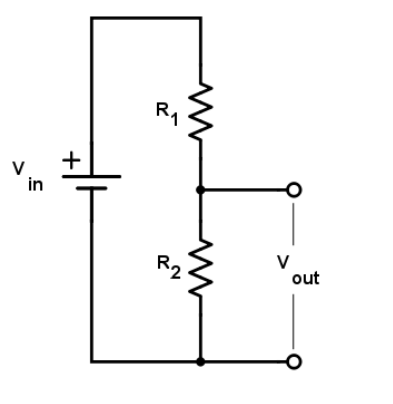
\includegraphics[width=0.6\textwidth]{voltage_divider.png}
   \caption{General voltage divider diagram}
\end{figure} 
The relation between \(V{in}\) and \(V{out}\) can be derived from the basic electric circuit relation. Whic is \(V{out}\) = \(V{in} \times \frac{R_2}{R_1+R_2}\) . So the have half of the voltage two of the 1k\(\Omega\) resistor is used.
As a result, voltage is divided, but to hold this relation, the current coming from the branch of \(R_1\) should be equal to the current going through the branch of \(R_2\). If we directly connect this output terminal to the summing configuration, the current would go through the \(R_2\) and \(R_f\) resistors of the summing circuit. Therefore it is needed to isolate those circuits. The buffer circuit explained in part b of step 2  is set. 
\subsubsection{a.}
%description script
Using the voltage divider and buffer circuitry, the signal is propagated to the summing circuit. The plot of \(V_{a} , V_{b} , V_{o} \) against \( Time\) is obtained using the signal value of \(V_{a}(t) = 2 V_{b}(t) = 4sin(1000\pi t) V\) . The plot is obtained as given in Figure 19.
%Figure 19 plot sum a\
\begin{figure}[H]
	\centering
   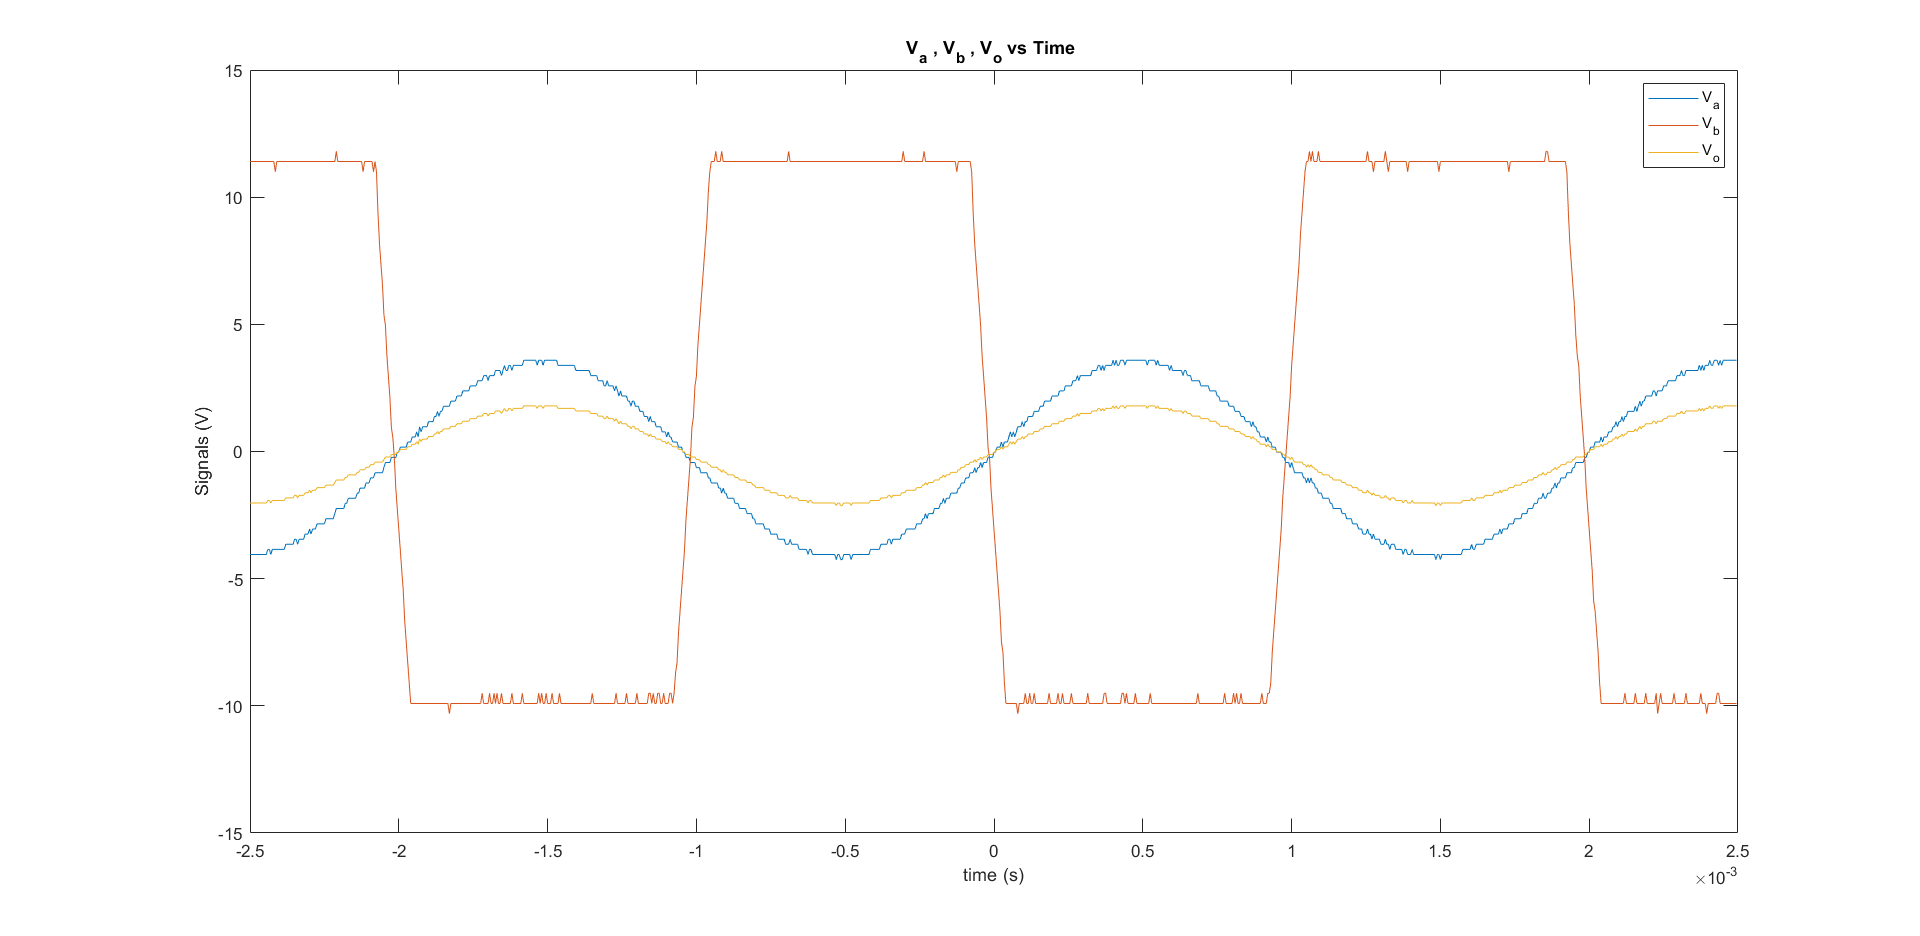
\includegraphics[width=1\textwidth]{e_3_a.png}
   \caption{\(V_{a} , V_{b} , V_{o} \) vs \( Time\)}
\end{figure} 
As a result, it can be said that the signals are summed and amplified. But, after excessing the linear region, output signal is saturated. Which means the voltage given from the supply pins determines the saturation regions.

\subsubsection{b.}
%description script
Using the voltage divider and buffer circuitry, the signal is supplied to the summing circuit. The plot of \(V_{a} , V_{b} , V_{o} \) against \( Time\) is obtained using the signal value of \(V_{a}(t) = 2 V_{b}(t) = 2sin(1000\pi t) V\) . The plot is obtained as given in Figure 20.
%Figure 20 plot sum b
\begin{figure}[H]
	\centering
   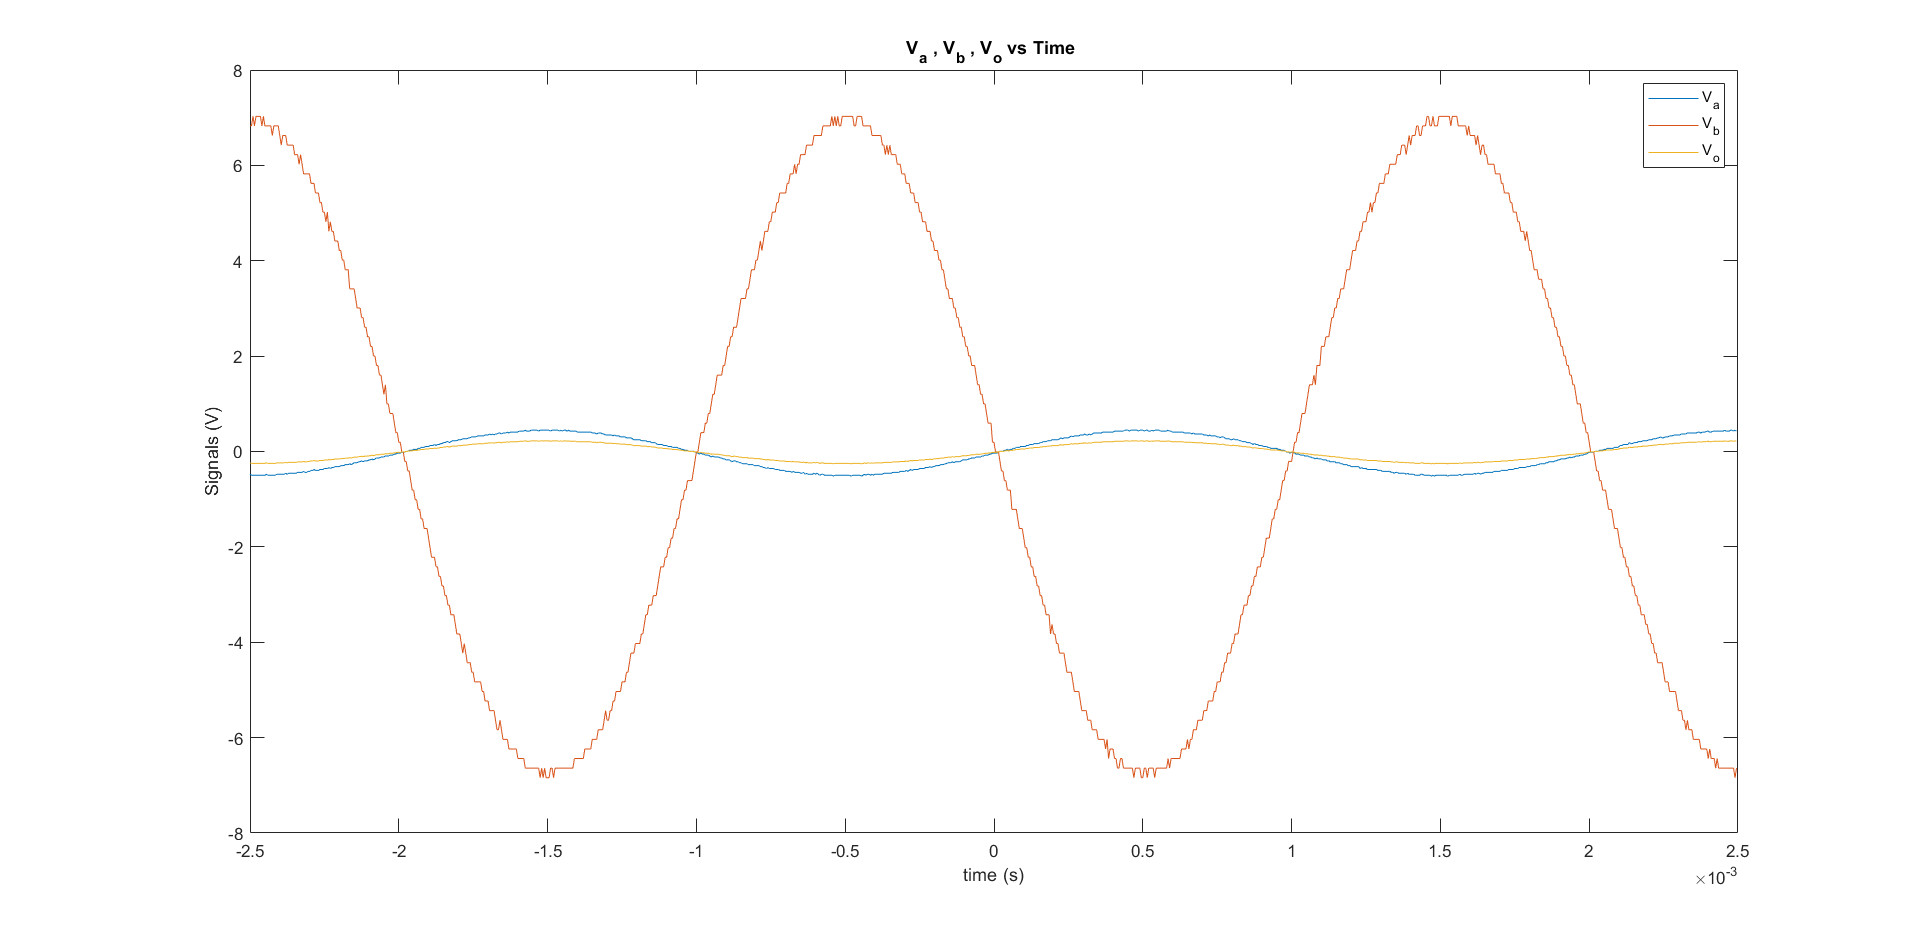
\includegraphics[width=1\textwidth]{e_3_b.png}
   \caption{\(V_{a} , V_{b} , V_{o} \) vs \( Time\)}
\end{figure} 
As a result, it can be said that the signals are summed and amplified. But, in this setup, the output signal is not saturated.

%Figure 21 comparison simulation res
Summing amplifier circuit is constructed in LTSpice environment with the values of \(V_{a}(t) = 2 V_{b}(t) = 4sin(1000\pi t) V\) . The schematic is given in the Figure 21. 
\begin{figure}[H]
	\centering
   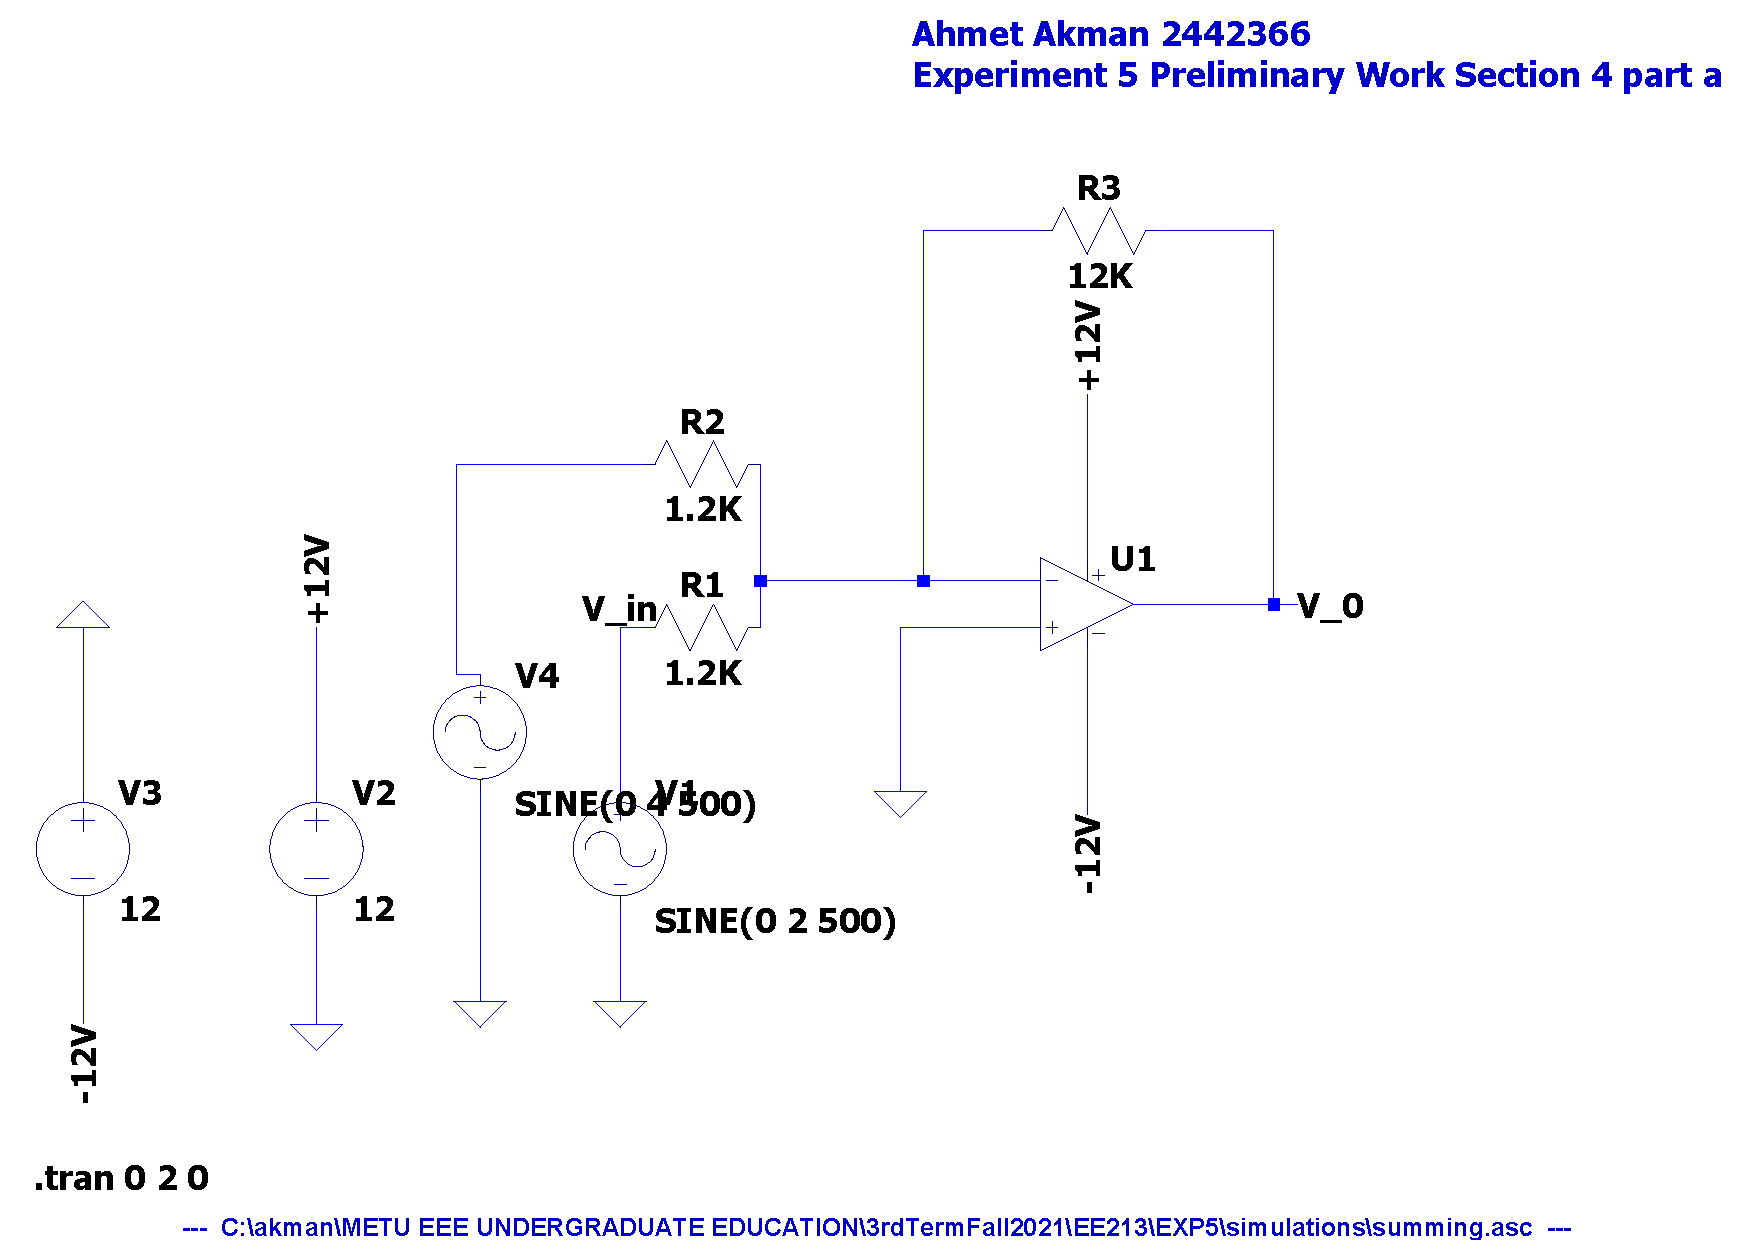
\includegraphics[width=0.8\textwidth]{summing_SCH.pdf}
   \caption{Circuit schematic for the summing amplifier.}
\end{figure} 
Then plot given in Figure 22 is obtained.
\begin{figure}[H]
	\centering
   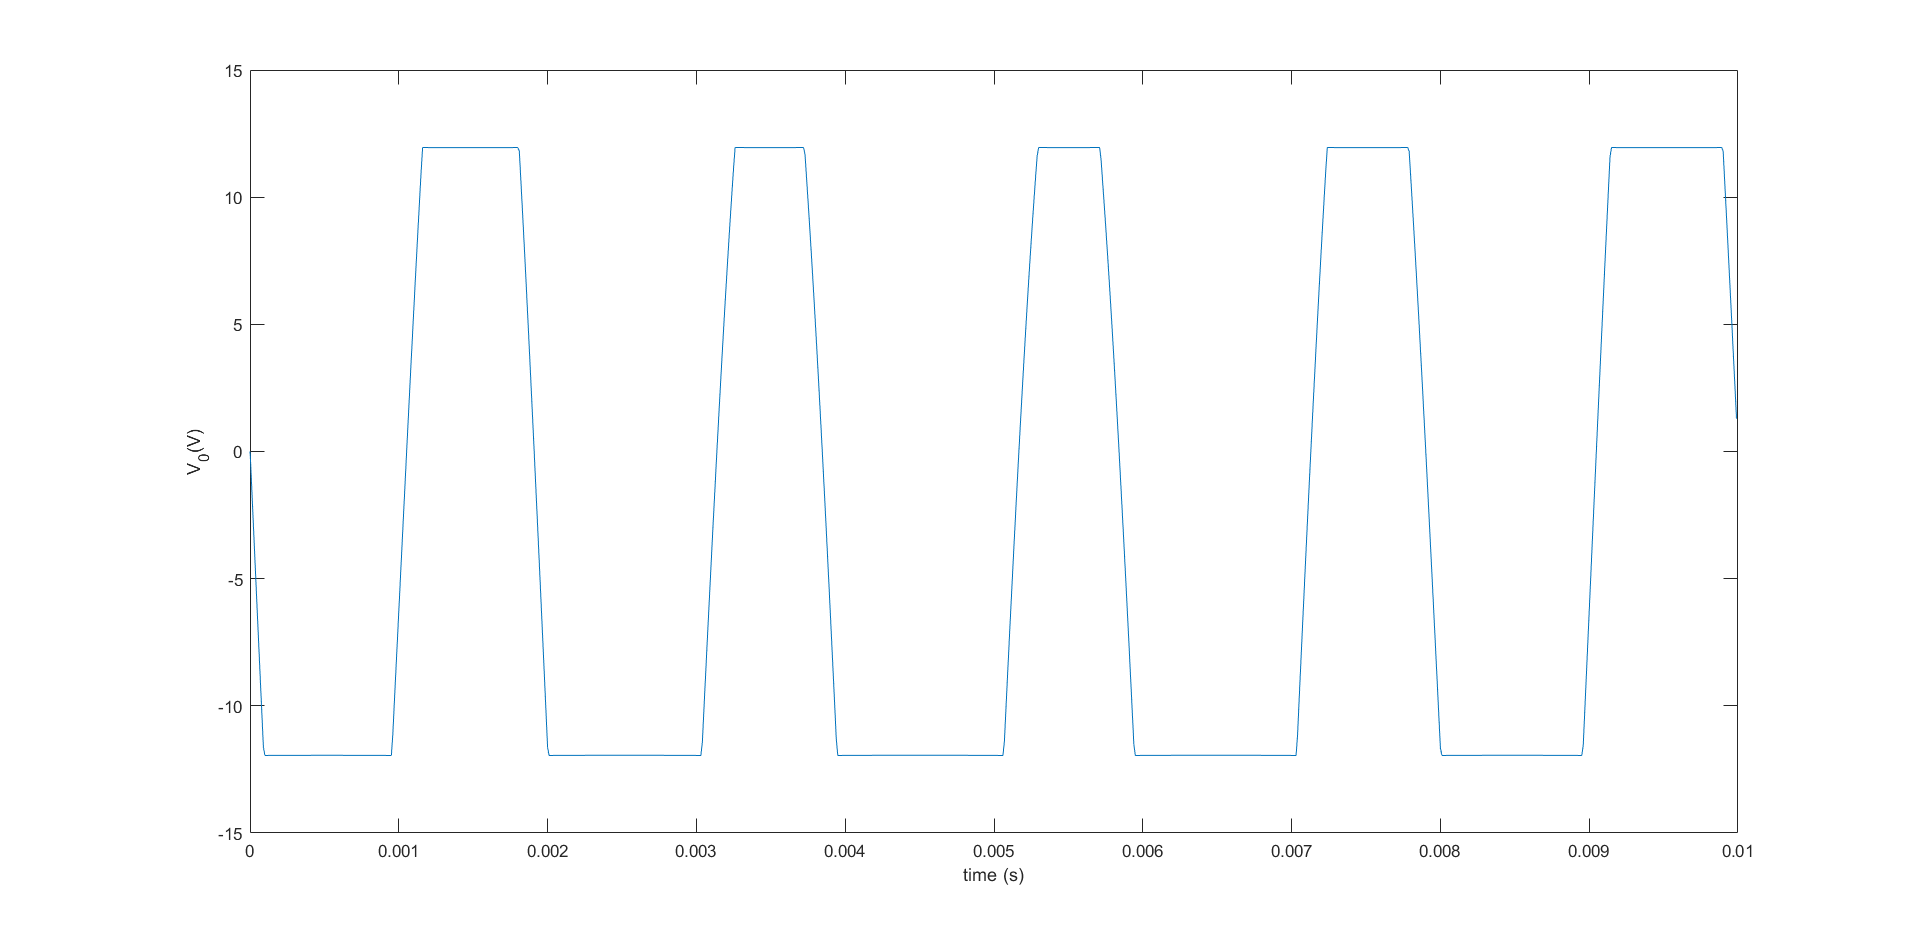
\includegraphics[width=1\textwidth]{4a_vs_t.png}
   \caption{\(V_0\) vs t}
\end{figure}
As a result, we obtained the behavior of \(V_0\) quite close to Figure 19.  Yet, the negative saturation region of the real circuit is slightly greater. This is expected to be stemmed from the non-ideality of either the LM741 component or the negative power line of the power supply.


\section{Conclusion}
In conclusion, in experiment 5, "Operational Amplifiers," as students, we have learned how basic circuit setups of Op-Amps can be constructed. Preliminary laboratory work is done via simulations of the basic Op-Amp circuits in an LTSpice environment. As students, we have observed different characteristics of Op-Amp comparator, buffer, non-inverting, inverting, and summing configurations, and we have learned how voltage divider should be used when there is a load to the output terminal. To sum up,in this experiment, as students, we have experimented with how operates different kinds of operational amplifier circuits and how to work with voltage dividers. 
\section*{Appendix I}
Total time spent on/during:
\begin{itemize}
	\item Pre-lab preparation: 6 hours (including the preliminary work and simulations) 
	\item Experimental work: 2 hours (hours spent in lab)
	\item Report writing: 6 hours 
\end{itemize}
\section*{Appendix II}
The outputs of the simulations are fetched from LTSpice and plotted in MATLAB.
%++++++++++++++++++++++++++++++++++++++++
% References section will be created automatically 
% with inclusion of "thebibliography" environment
% as it shown below. See text starting with line
% \begin{thebibliography}{99}
% Note: with this approach it is YOUR responsibility to put them in order
% of appearance.

%\begin{thebibliography}{99}

%https://tr.overleaf.com/latex/templates/sample-lab-report-for-u-of-r-phys-349/pgsyqngcyjxk

%\end{thebibliography}


\end{document}


\begin{table}[H]
	\begin{center}
		\caption{Resistance reading by color code convention.}
		\vspace{2mm}
		\begin{tabular}{||c | c | c||} 
		 \hline
		 Color Order & Value & Tolerance \\ [0.5ex] 
		 \hline\hline
		 Brown / Black / Red / Gold & 1k\( \Omega \) & \( \% \) 5  \\ 
		 \hline
		 Yellow / Violet / Red / Gold & 4.7k\( \Omega \) & \( \% \) 5   \\
		 \hline
		 Brown / Grey / Orange / Gold & 18k\( \Omega \) & \( \% \) 5  \\ [1ex] 
		 \hline
		\end{tabular}
	\end{center}
	\end{table}

	\begin{figure}[H]
 		\centering
		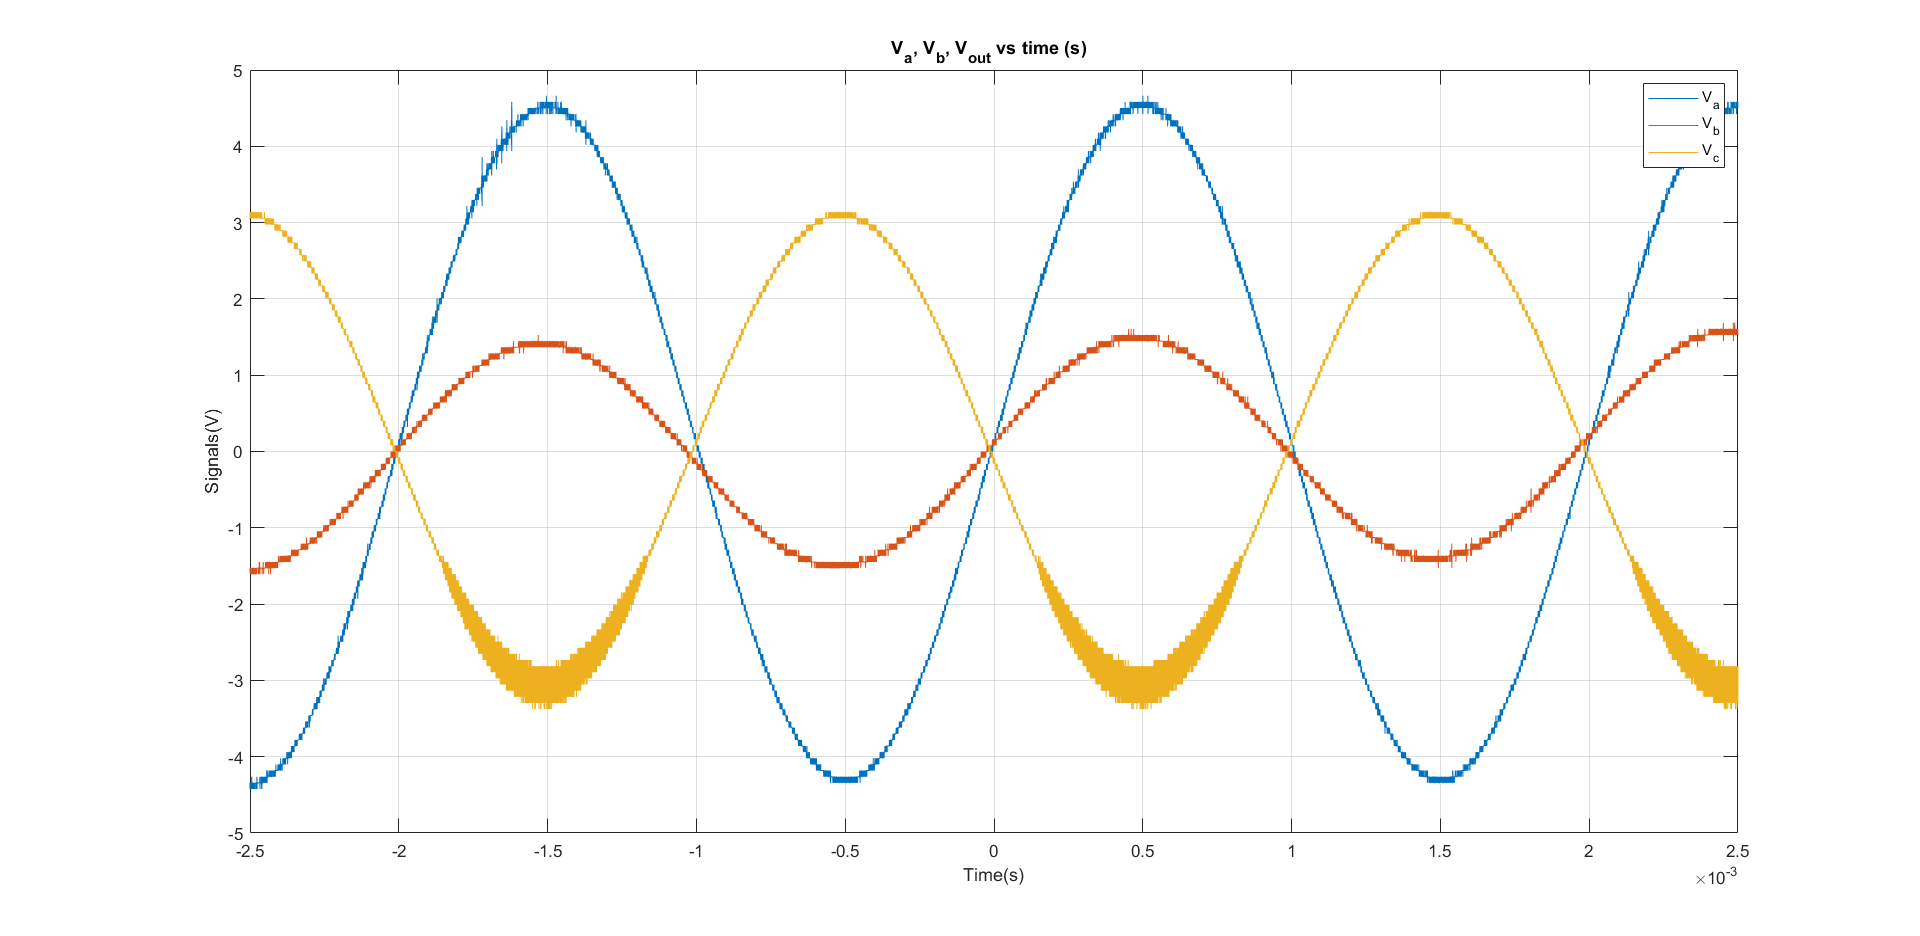
\includegraphics[width=0.6\textwidth]{5.png}
		\caption{Circuit schematic for the step 5}
	\end{figure} 

	\begin{figure}[htp] \centering{
		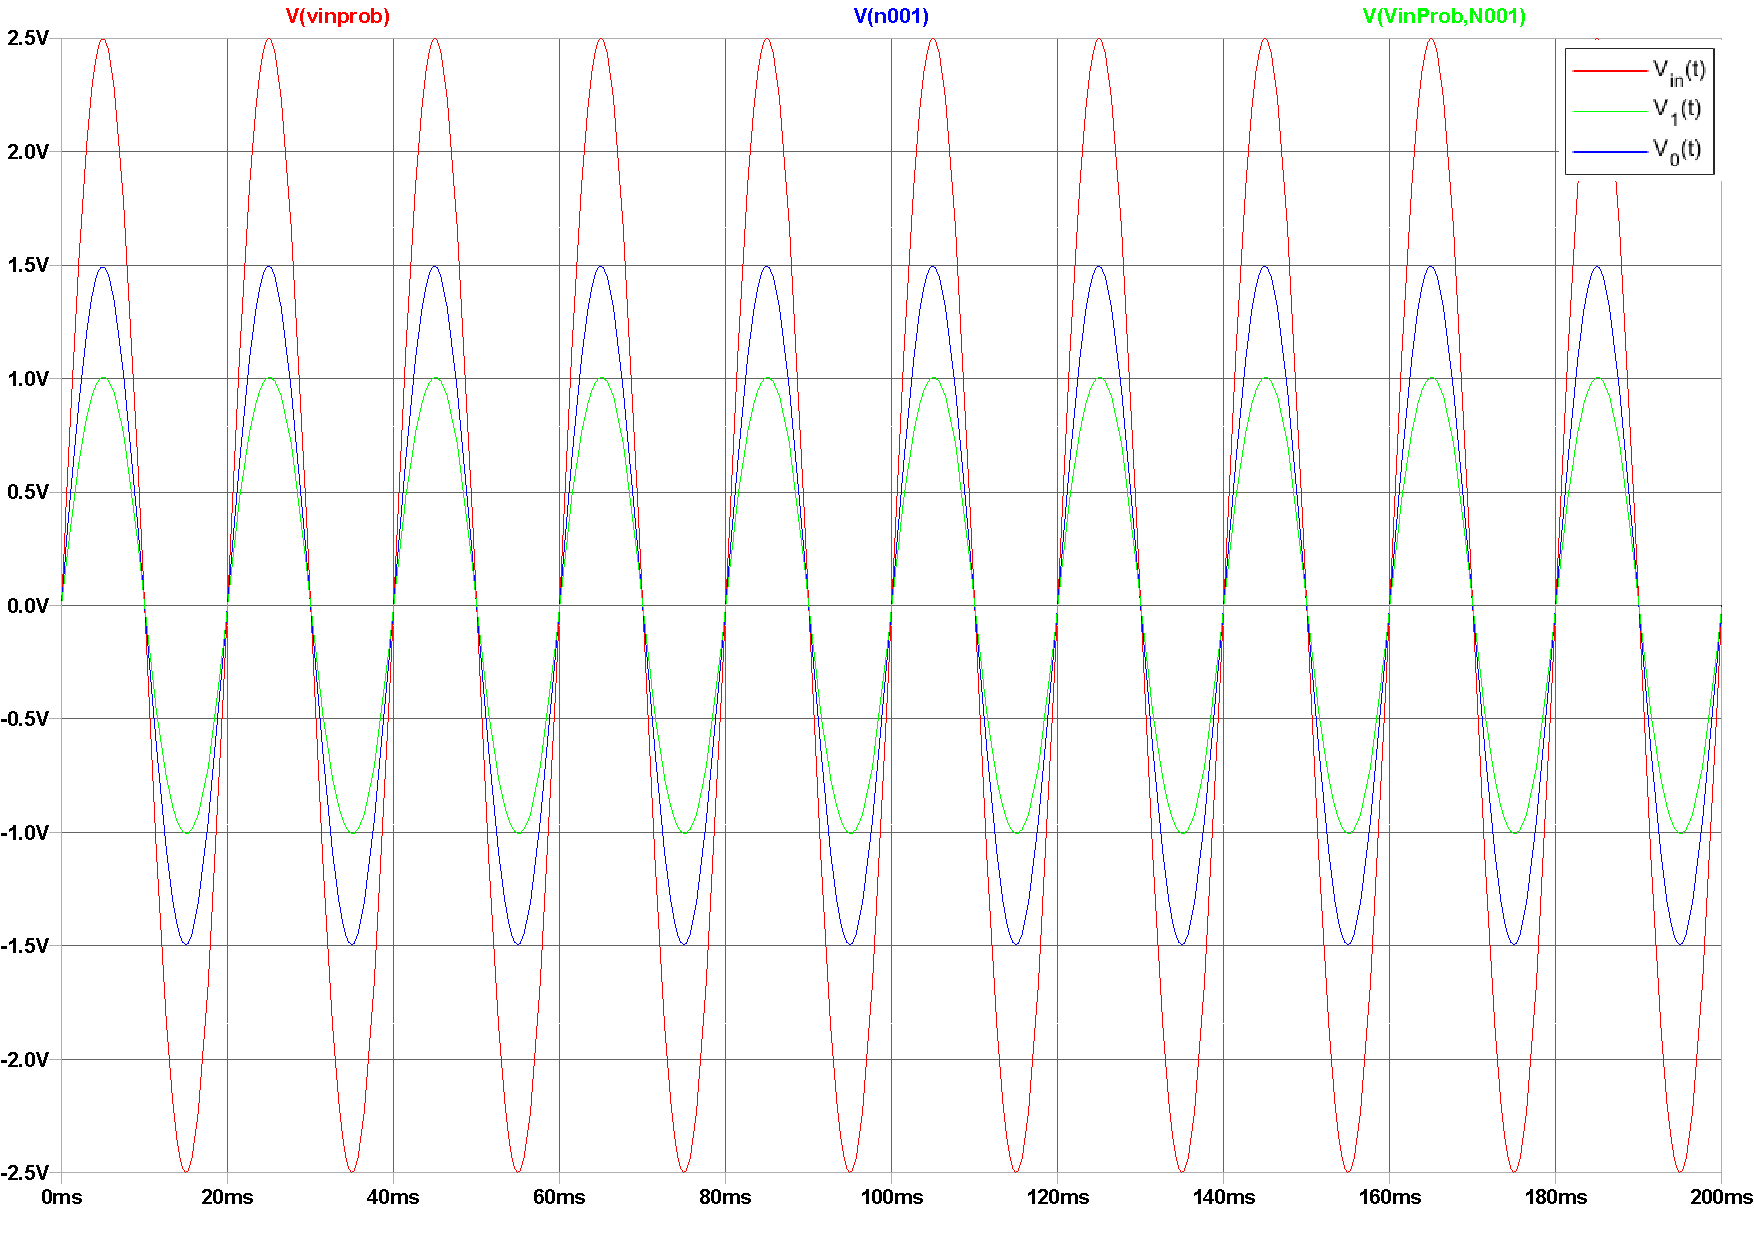
\includegraphics[scale=0.25]{2a_plot.pdf}}
		\caption{Experiment 2}
\end{figure}
	